\documentclass{article}
\usepackage{indentfirst}
\usepackage{multirow}\usepackage{makecell}\usepackage{diagbox}
\setlength{\parindent}{2em}
\usepackage{xeCJK}\usepackage{float}
\usepackage{xcolor}\usepackage{tcolorbox}
\usepackage{colortbl}
\usepackage{graphicx}
\usepackage{subfig}
\setCJKmainfont{SimSun} 
\usepackage{tikz}            % 添加 TikZ 包以支持 tikzpicture 环境
\usepackage{pgfplots}        % 核心绘图包
\usepgfplotslibrary{patchplots}
\pgfplotsset{compat=1.17}
\usepackage{amsmath}
\usetikzlibrary{calc}
\usepackage{amssymb}
\usepackage{amsthm}
\usepackage{geometry}
\usepackage{tocbibind}
\usepackage{hyperref}
\usepackage{enumitem}
\geometry{a4paper,margin=2.5cm}


\title{数列复习学案(天津专用)}
\author{小白高考数学}
\date{}

\hypersetup{
    colorlinks=true,    % 链接文字上色（false则加边框）
    linkcolor=black,     % 目录跳转链接颜色（黑色）
    urlcolor=blue,      % 网址链接颜色
    citecolor=green,    % 引用链接颜色
    bookmarks=true,     % 生成PDF书签（侧边栏）
    bookmarksnumbered=true, % 书签显示章节号
    pdfstartview=FitH   % PDF打开时自适应宽度
}

\renewcommand{\contentsname}{目录}
\begin{document}
\maketitle

\vspace{30\baselineskip}
\begin{center}
迟序之数，非出神怪，有形可检，有数可推
\end{center}
\begin{flushright}
    \rightskip=7em 
——祖冲之《缀术》
\end{flushright}    
\newpage
\tableofcontents % 核心命令：生成目录
\newpage 

\section{知识要点}
\subsection{数列的概念与性质}
\subsubsection{数列的基本概念}
一般地，我们把按照确定的顺序排列的一列数称为\textcolor{cyan}{数列}（sequence of number），数列中的每一个数叫做这个数列的\textcolor{cyan}{项}。数列的第一个位置上的数叫做这个数列的第1项，常用符号 \(a_1\) 表示，第二个位置上的数叫做这个数列的第2项，用 \(a_2\) 表示……第 \(n\) 个位置上的数叫做这个数列的第 \(n\) 项，用 \(a_n\) 表示。其中第1项也叫做\textcolor{cyan}{首项}。①是按年龄从小到大的顺序排列的，②是按每月的日期从小到大的顺序排列的，③是按幂指数从小到大的顺序排列的，它们都是从第1项开始的。

数列的一般形式是
\[
a_1,\ a_2,\ \dots,\ a_n,\ \dots,
\]
简记为 \(\{a_n\}\).

由于数列$\{a_n\}$中的每一项$a_n$与它的序号$n$有下面的对应关系：

\[
\begin{array}{c*{6}{c}}
\text{序号} & 1 & 2 & 3 & \cdots & n & \cdots \\
           & \downarrow & \downarrow & \downarrow & & \downarrow & \\
\text{项}   & a_1 & a_2 & a_3 & \cdots & a_n & \cdots
\end{array}
\]

所以数列$\{a_n\}$是从正整数集$\mathbf{N}^*$（或它的有限子集$\{1,2,\dots,n\}$）到实数集$\mathbf{R}$的函数，其自变量是序号$n$，对应的函数值是数列的第$n$项$a_n$，记为$a_n = f(n)$。也就是说，当自变量从$1$开始，按照从小到大的顺序依次取值时，对应的一列函数值$f(1),f(2),\dots,f(n),\dots$就是数列$\{a_n\}$。

另一方面，对于函数$y = f(x)$，如果$f(n)$（$n \in \mathbf{N}^*$）有意义，那么
\[
f(1),\ f(2),\ \dots,\ f(n),\ \dots
\]
构成了一个数列$\{f(n)\}$。

\begin{tcolorbox}[colback=blue!10,colframe=blue!70!black,title=]
以前我们学过的函数的自变量通常是连续变化的，而数列是自变量为离散的数的函数。
\end{tcolorbox}

要想展现一个确定的数列，我们需要给出它的项数和每一项的表达式，这就是通项公式。数列$\{a_n\}$的通项公式是一个关于$n$的表达式，满足当$n$取正整数值时，表达式的值等于数列的第$n$项$a_n$。例如，数列$\{a_n\}$的通项公式为$a_n = 2n + 1$，则当$n=1$时，$a_1 = 2(1) + 1 = 3$；当$n=2$时，$a_2 = 2(2) + 1 = 5$；当$n=3$时，$a_3 = 2(3) + 1 = 7$……以此类推，我们可以得到数列$\{a_n\}$的前几项为：3, 5, 7, ……

当然，与通项公式式相对应的还有递推公式。数列$\{a_n\}$的递推公式是一个关于数列项之间关系的表达式，满足当$n$取正整数值时，表达式的值等于数列的第$n$项$a_n$。例如，数列$\{a_n\}$的递推公式为$a_n = a_{n-1} + 2$，且$a_1 = 3$，则当$n=2$时，$a_2 = a_{1} + 2 = 3 + 2 = 5$；当$n=3$时，$a_3 = a_{2} + 2 = 5 + 2 = 7$……以此类推，我们可以得到数列$\{a_n\}$的前几项为：3, 5, 7, ……

同时，数列的前n项和也是一个重要的概念。数列$\{a_n\}$的前n项和是指数列的前n项的和，记为$S_n$，即
\[S_n = a_1 + a_2 + \cdots + a_n.\]例如，数列$\{a_n\}$的通项公式为$a_n = 2n + 1$，则当$n=1$时，$S_1 = a_1 = 2(1) + 1 = 3$；当$n=2$时，$S_2 = a_1 + a_2 = 2(1) + 1 + 2(2) + 1 = 5$；当$n=3$时，$S_3 = a_1 + a_2 + a_3 = 2(1) + 1 + 2(2) + 1 + 2(3) + 1 = 7$……以此类推，我们可以得到数列$\{a_n\}$的前几项为：3, 5, 7, ……

\begin{tcolorbox}[colback=blue!10,colframe=blue!70!black,title=]
一个数列的三种公式：通项公式、递推公式和前n项和公式之间的转化是数列研究的核心问题之一,其中通项公式是最重要的桥梁。具体而言，用前n项和公式求解得到通项公式是容易的，这是因为
$$a_n=S_n-S_{n-1}$$

不过需要注意的是$a_1$是需要单独验证的，这是因为$S_0$没有定义。当然，从通项公式得到递推公式也是容易的，例如我们将$a_n$和$a_{n-1}$做差，就能得到：

$$a_n=a_{n-1}+f(n)$$

其中$f(n)$是一个关于$n$的函数，这就是数列$\{a_n\}$的递推公式，当然，一个确定数列的通项公式未必唯一，换言之，不同的通项公式可能导向同一个数列。

至于，从递推公式得到通项公式，从通向公式得到求和式都是比较困难的问题，这两种问题我们再后面分条解决。
\end{tcolorbox}

\newpage
\subsubsection{数列的周期性}

一般地，对于数列$\{a_n\}$，若有$a_{n+k} = a_n$（$n \in \mathbf{N}^*, k \in \mathbf{N}^*$），则该数列为{周期数列}，且周期为$k$。
要判断一个数列是否具有周期性，主要方法是利用递推公式求出数列的若干项，观察得到规律或由递推公式直接推导出 \(a_n = a_{n+k}\)。我们来看一个例子来进一步阐述之：

已知数列$\{a_n\}$满足$a_1 = -1$，$a_{n+1} = \dfrac{1}{1 - a_n}$，求$a_{2024}$的值：我们先计算几项$a_1 = -1$，$a_2 = \dfrac{1}{1 - a_1} = \dfrac{1}{1 - (-1)} = \dfrac{1}{2}$，$a_3 = \dfrac{1}{1 - a_2} = \dfrac{1}{1 - \dfrac{1}{2}} = 2$，$a_4 = \dfrac{1}{1 - a_3} = \dfrac{1}{1 - 2} = -1$……以此类推，我们可以得到数列$\{a_n\}$的前几项为：-1, $\dfrac{1}{2}$, 2, -1, $\dfrac{1}{2}$, 2, ……我们发现数列$\{a_n\}$的第4项又回到了-1，这说明数列$\{a_n\}$具有周期性，且周期为3

事实上，我们计算到第四项就已经可以知道数列$\{a_n\}$的周期性了，因为此数列的递推公式是一个不含$n$的表达式，因此决定数列后一项的值只是前一项的数值，而与这是数列的第几项无关。

\subsubsection{数列的单调性}
数列$\{a_n\}$的单调性是指数列的项随着序号的增大而单调增加或单调减少。具体而言，如果对于任意的$n \in \mathbf{N}^*$，都有$a_{n+1} > a_n$，则数列$\{a_n\}$是单调递增的；如果对于任意的$n \in \mathbf{N}^*$，都有$a_{n+1} < a_n$，则数列$\{a_n\}$是单调递减的。

判断数列单调性的方法有：

\begin{enumerate}
\item 做差法：计算数列的相邻两项之差，即$a_{n+1} - a_n$，如果对于任意的$n \in \mathbf{N}^*$，都有$a_{n+1} - a_n > 0$，则数列$\{a_n\}$是单调递增的；如果对于任意的$n \in \mathbf{N}^*$，都有$a_{n+1} - a_n < 0$，则数列$\{a_n\}$是单调递减的。
\item 做商法：计算数列的相邻两项之比，即$a_{n+1} / a_n$，如果对于任意的$n \in \mathbf{N}^*$，都有$a_{n+1} / a_n > 0$，则数列$\{a_n\}$是单调递增的；如果对于任意的$n \in \mathbf{N}^*$，都有$a_{n+1} / a_n < 0$，则数列$\{a_n\}$是单调递减的。当然，此时要注意两点：一是数列中不能含有0项；二是这种方法只能判别正数数列（或复数数列，此时结论相反），对于同时有负数和正数的数列，相邻两项的比值可能是一个负值，这就无法说清了。
\item 函数拟合法：如果数列$\{a_n\}$的通项公式可以表示为一个关于$n$的函数$f(n)$，我们可以通过研究函数$f(x)$的单调性来判断数列$\{a_n\}$的单调性。具体而言，如果函数$f(x)$在定义域内是单调递增的，那么数列$\{a_n\}$也是单调递增的；如果函数$f(x)$在定义域内是单调递减的，那么数列$\{a_n\}$也是单调递减的。当然，我们需要注意的是数列只体现了函数在正整数上的取值情况，因此函数的一些“小曲折”可能会被数列“过滤掉”，因此我们需要仔细分析函数的单调性，不能仅仅通过函数的图像来判断数列的单调性。
\end{enumerate}
    
 


当然，始终单调递增或者是单调递减的数列是不多的，更多的时候需要我们去研究一个数列的增减情况，进而探究其最大（最小）值。下面我们通过一个例题来说明求数列最大（最小）值的方法：
\vspace{2\baselineskip}

\noindent\textbf{[典例]：} 已知数列$\{a_n\}$的通项公式是$a_n = (n+2)\times\left(\frac{7}{8}\right)^n (n\in \mathbf{N}^*)$，试问数列$\{a_n\}$是否有最大项？若有，求出最大项；若没有，说明理由。

\bigskip

\noindent\textbf{[解析]：} 

\quad \textbf{方法一（作差法）}
\[
\begin{aligned}
a_{n+1} - a_n &= (n+3)\times\left(\frac{7}{8}\right)^{n+1} - (n+2)\times\left(\frac{7}{8}\right)^n \\
&= \left(\frac{7}{8}\right)^n \times \frac{5-n}{8}.
\end{aligned}
\]

当$n < 5$时，$a_{n+1} - a_n > 0$，即$a_{n+1} > a_n$；

当$n = 5$时，$a_{n+1} - a_n = 0$，即$a_{n+1} = a_n$；

当$n > 5$时，$a_{n+1} - a_n < 0$，即$a_{n+1} < a_n$。

故$a_1 < a_2 < a_3 < a_4 < a_5 = a_6 > a_7 > a_8 > \cdots$，

所以数列$\{a_n\}$有最大项，最大项为$a_5$和$a_6$，且
\[
a_5 = a_6 = \frac{7^6}{8^5}.
\]

\quad \noindent\textbf{方法二（作商法）}

因为 \(a_n = (n+2)\times\left(\frac{7}{8}\right)^n\)（\(n\in \mathbf{N}^*\)），所以 \(a_n > 0\)，
\[
\frac{a_{n+1}}{a_n} = \frac{(n+3)\times\left(\frac{7}{8}\right)^{n+1}}{(n+2)\times\left(\frac{7}{8}\right)^n}
= \frac{7(n+3)}{8(n+2)}.
\]

令 \(\frac{a_{n+1}}{a_n} > 1\)，解得 \(n < 5\)；

令 \(\frac{a_{n+1}}{a_n} = 1\)，解得 \(n = 5\)；

令 \(\frac{a_{n+1}}{a_n} < 1\)，解得 \(n > 5\)。

故 \(a_1 < a_2 < a_3 < a_4 < a_5 = a_6 > a_7 > a_8 > \cdots\)，

所以数列 \(\{a_n\}\) 有最大项，最大项为 \(a_5\) 和 \(a_6\)，且
\[
a_5 = a_6 = \frac{7^6}{8^5}.
\]

\quad \noindent\textbf{方法三（不等式组法）}
假设$\{a_n\}$中有最大项，且最大项为第$n$项，则
\[
\begin{cases}
a_n \ge a_{n-1}, \\
a_n \ge a_{n+1},
\end{cases}
\]
即
\[
\begin{cases}
(n+2)\times\left(\frac{7}{8}\right)^n \ge (n+1)\times\left(\frac{7}{8}\right)^{n-1}, \\
(n+2)\times\left(\frac{7}{8}\right)^n \ge (n+3)\times\left(\frac{7}{8}\right)^{n+1},
\end{cases}
\]
解得
\[
\begin{cases}
n \le 6, \\
n \ge 5,
\end{cases}
\]
即$5 \le n \le 6$。

故数列$\{a_n\}$有最大项，最大项为$a_5$和$a_6$，且
\[
a_5 = a_6 = \frac{7^6}{8^5}.
\]

\noindent\textbf{[反思]：} 

这三种方法本质上并未差别，都是通过不等式的求解来说明：数列中何时后一项大于前一项，何时后一项小于前一项，这样便可找到数列的最大值。方法一二的区别只在于使用了上述不同的判别法。
其中，做差判别是通用的方法，做商的方法一般用于函数中出现指数型的结构时，至于方法三，不过是取到最大值时的$n$设出来罢了，本质无出其右。
\vspace{2\baselineskip}
\newpage

\begin{center}
    \textbf{微专题：数列递推公式求通项公式的一个方法：累加、累乘法}
\end{center}

对于能化简成$a_{n+1} - a_n = f(n)$的递推公式，我们可以通过累加法来求解数列的通项公式；对于能化简成$\dfrac{a_{n+1}}{a_n} = f(n)$的递推公式，我们可以通过累乘法来求解数列的通项公式.
具体步骤我们通过两道例题来说明：
\vspace{2\baselineskip}

\noindent\textbf{例题： } 在数列$\{a_n\}$中，$a_1 = 2$，$a_{n+1} = a_n + \ln\left(1 + \frac{1}{n}\right)$，则数列$\{a_n\}$的通项公式为(\;\;\;)

\vspace{1em}
A. $2 + \ln n$ \quad
B. $2 + (n-1)\ln n$ \quad
C. $2 + n\ln n$ \quad
D. $1 + n + \ln n$

\bigskip

\noindent\textbf{[累加法]}
\[
a_{n+1} - a_n = \ln\left(1 + \frac{1}{n}\right) = \ln\frac{1+n}{n} = \ln(1+n) - \ln n,
\]

\[
\begin{aligned}
a_1 &= 2, \\
a_2 - a_1 &= \ln 2, \\
a_3 - a_2 &= \ln 3 - \ln 2, \\
a_4 - a_3 &= \ln 4 - \ln 3, \\
&\cdots, \\
a_n - a_{n-1} &= \ln n - \ln(n-1) \quad (n \ge 2),
\end{aligned}
\]

以上各式相加得
\[
a_n = 2 + \ln 2 + (\ln 3 - \ln 2) + \cdots + \left[\ln n - \ln(n-1)\right],
\]

所以 $a_n = 2 + \ln n \ (n \ge 2)$。

因为 $a_1 = 2$ 也适合上式，所以 $a_n = 2 + \ln n$。（注意$a_1$要特别验证，因为无论是累加法还是累乘法，都是以$a_1$为起点的，只有$a_1$确定了，后面的值才能随着确定。）

\vspace{2\baselineskip}

\noindent\textbf{例题： } 已知数列$\{a_n\}$中，$a_1 = 1$，$a_n = n(a_{n+1} - a_n)$（$n \in \mathbf{N}^*$）。求数列$\{a_n\}$的通项公式。

\bigskip

\noindent\textbf{[累乘法]}

因为$ a_n = n(a_{n+1} - a_n)$，$a_n \neq 0$，即
\[
\frac{a_{n+1}}{a_n} = \frac{n+1}{n},
\]

\begin{tcolorbox}[colback=blue!10,colframe=blue!70!black,title=]
\textbf{[易错点]} 用累乘法时，注意数列中的项不为0
\end{tcolorbox}

\[
\therefore \frac{a_2}{a_1} = \frac{2}{1},\ \frac{a_3}{a_2} = \frac{3}{2},\ \frac{a_4}{a_3} = \frac{4}{3},\ \dots,\ \frac{a_n}{a_{n-1}} = \frac{n}{n-1}\ (n \ge 2).
\]

以上各式两边分别相乘，得
\[
\frac{a_n}{a_1} = \frac{2}{1} \times \frac{3}{2} \times \frac{4}{3} \times \cdots \times \frac{n}{n-1} = n.
\]

又 $a_1 = 1$，$\therefore a_n = n\ (n \ge 2)$。

$\because a_1 = 1$ 也适合上式，

$\therefore a_n = n$。

\newpage

\begin{center}
    小节练习
\end{center}

\noindent\textbf{例一：} （课本原题）写出下列数列的前 10 项，并作出它们的图象：
\begin{enumerate}
    \item 素数按从小到大的顺序排列成的数列；
    \item 欧拉函数 $\varphi(n)$（$n\in \mathbf{N}^*$）的函数值按自变量从小到大的顺序排列成的数列。
\end{enumerate}

\begin{tcolorbox}[colback=blue!10,colframe=blue!70!black,title=]
欧拉函数 $\varphi(n)$（$n\in \mathbf{N}^*$）的函数值等于所有不超过正整数 $n$，且与 $n$ 互素（此数学概念为小学所学，中学阶段并未涉及，不过2022年的新高考一卷确实考到了此概念）的正整数的个数，例如，$\varphi(1)=1$，$\varphi(4)=2$。
\end{tcolorbox}
\vspace{10\baselineskip}

\noindent\textbf{例二：} （课本原题）已知函数 \(f(x) = \frac{2^x - 1}{2^x}\)（\(x \in \mathbf{R}\)），设数列 \(\{a_n\}\) 的通项公式为 \(a_n = f(n)\)（\(n \in \mathbf{N}^*\)）。

\begin{enumerate}
    \item 求证 \(a_n \ge \frac{1}{2}\)。
    \item \(\{a_n\}\) 是递增数列还是递减数列？为什么？
\end{enumerate}
\vspace{15\baselineskip}

\noindent\textbf{例三： }（2024天津市南开区质检）已知数列$\{a_n\}$的通项公式为$a_n = n^2 + tn$，若数列$\{a_n\}$为递增数列，求$t$的取值范围
\newpage

\noindent\textbf{例四： } 已知数列$\{a_n\}$中，$a_1 = 1$，前$n$项和$S_n = \dfrac{n+2}{3}a_n$，求数列的通项公式。
\vspace{15\baselineskip}

\noindent\textbf{例五： }（2022全国乙卷）嫦娥二号卫星在完成探月任务后，继续进行深空探测，成为我国第一颗环绕太阳飞行的人造行星。为研究嫦娥二号绕日周期与地球绕日周期的比值，用到数列$\{b_n\}$：
\[
b_1 = 1 + \frac{1}{\alpha_1},\quad
b_2 = 1 + \frac{1}{\alpha_1 + \frac{1}{\alpha_2}},\quad
b_3 = 1 + \frac{1}{\alpha_1 + \frac{1}{\alpha_2 + \frac{1}{\alpha_3}}},\quad \dots,
\]
依此类推，其中 $\alpha_k \in \mathbf{N}^*$（$k=1,2,\dots$）。则

\vspace{1em}
A. $b_1 < b_5$ \quad
B. $b_3 < b_8$ \quad
C. $b_6 < b_2$ \quad
D. $b_4 < b_7$
\vspace{5\baselineskip}

\noindent\textbf{例六： }（2021北京）数列$\{a_n\}$是递增的整数数列，且$a_1 \ge 3$，$a_1 + a_2 + a_3 + \dots + a_n = 100$，则$n$的最大值为

\vspace{1em}
A. 9 \quad
B. 10 \quad
C. 11 \quad
D. 12
\vspace{5\baselineskip}

\noindent\textbf{例七： }（全国三卷）设数列$\{a_n\}$满足
\[
a_1 + 3a_2 + \dots + (2n-1)a_n = 2n.
\]

\vspace{1em}
\begin{enumerate}
    \item 求$\{a_n\}$的通项公式；
    \item 求数列$\left\{\frac{a_n}{2n+1}\right\}$的前$n$项和。
\end{enumerate}
\newpage

\subsection{等差数列}
\subsubsection{等差数列的性质}

一般地，如果一个数列从第 2 项起，每一项与它的前一项的差都等于同一个常数，那么这个数列就叫做\textcolor{cyan}{等差数列}（arithmetic progression），这个常数叫做等差数列的\textcolor{cyan}{公差}（common difference），公差通常用字母 \(d\) 表示。
等差数列的定义可用数学符号语言描述为：$a_n - a_{n-1} = d$ 对任意的 $n \ge 2, n \in \mathbf{N}^*$ 均成立，或 $a_{n+1} - a_n = d$ 对任意的 $n \in \mathbf{N}^*$ 均成立，其中 $d$ 为常数。
\vspace{2\baselineskip}

知识点 1. 形式：
\[
\begin{cases}
\text{通项} & a_n = a_1 + (n-1)d \quad \text{（$a_1$为首项，$d$为公差）}, \\
\text{递推} & a_{n+1} - a_n = d, \\
\text{求和} & S_n = an^2 + bn \quad \left(\text{其中 } a = \frac{d}{2},\ b = \frac{2a_1 - d}{2}\right).
\end{cases}
\]
\vspace{1\baselineskip}

知识点 2. 等差中项：若 \(a, S, b\) 成等差数列，则 \(S = \frac{a + b}{2}\)，我们称 \(S\) 为 \(a, b\) 的等差中项。
\vspace{1\baselineskip}

知识点 3. 等差数列的性质:若数列 \(\{a_n\}\) 是公差为 \(d\) 的等差数列，则有如下性质：：

\begin{enumerate}
    \item \(a_n = a_m + (n - m)d\)，\(d = \frac{a_n - a_m}{n - m}\ (n \neq m)\)；
    \item 若 \(m + n = p + q\)，则 \(a_m + a_n = a_p + a_q\)。
    \item 下标成等差数列的项 \(a_k, a_{k+m}, a_{k+2m}, \dots\) 组成以 \(md\) 为公差的等差数列。
    \item 数列 \(\{ta_n + \lambda\}\)（\(t, \lambda\) 是常数）是公差为 \(td\) 的等差数列。
    \item 若数列 \(\{b_n\}\) 为等差数列，则数列 \(\{ta_n \pm \lambda b_n\}\)（\(t, \lambda\) 是常数）仍为等差数列。
\end{enumerate}

知识点 4.等差数列与一次函数的关系：

由于 \(a_n = a_1 + (n-1)d = dn + (a_1 - d)\)，当 \(d \neq 0\) 时，等差数列 \(\{a_n\}\) 的第 \(n\) 项 \(a_n\) 是一次函数 \(f(x) = dx + (a_1 - d)\)（\(x \in \mathbf{N}^*\)）。当 \(x = n\) 时的函数值，即 \(a_n = f(n)\)。

因此，从图象上看，表示数列 \(\{a_n\}\) 的各点均匀分布在直线 \(f(x) = dx + (a_1 - d)\) 上。

反之，任给一次函数 \(f(x) = kx + b\)（\(k, b\) 为常数），则 \(f(1), f(2), \dots, f(n), \dots\) 构成一个等差数列 \(\{nk + b\}\)，其首项为 \(k + b\)，公差为 \(k\)。

从这个角度我们可以看出，等差数列的单调性取决于公差的符号。如果公差为正，则数列是递增的；如果公差为负，则数列是递减的。而这个公差对于到一次函数中，就是一次函数的斜率。

\begin{figure}[H]
    \centering
    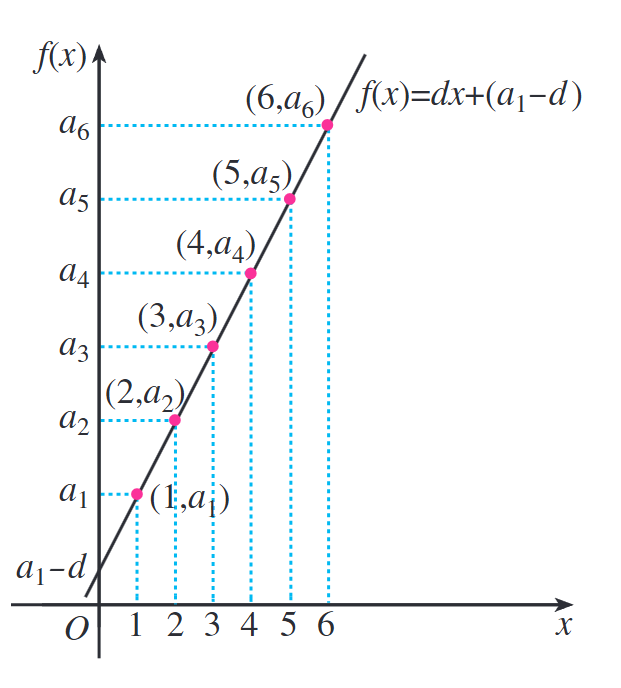
\includegraphics[width=0.4\textwidth]{1.png} % 不要加后缀 .jpg .png
\end{figure}

\newpage

\begin{tcolorbox}[colback=blue!10,colframe=blue!70!black,title=]

\noindent\textbf{判断一个数列是否为等差数列的方法}

1. 定义法
\[
a_{n+1} - a_n = d\ (n \in \mathbf{N}^*) \ \text{或} \ a_n - a_{n-1} = d\ (n \ge 2, n \in \mathbf{N}^*) \iff \text{数列}\{a_n\}\text{是等差数列}.
\]

2. 等差中项法
\[
2a_{n+1} = a_n + a_{n+2}\ (n \in \mathbf{N}^*) \iff \{a_n\}\ \text{为等差数列}.
\]

3. 通项公式法
\[
\text{数列}\{a_n\}\text{的通项公式形如}\ a_n = pn + q\ (p,q\ \text{为常数}) \iff \text{数列}\{a_n\}\text{为等差数列}.
\]

\end{tcolorbox}

\subsubsection{等差数列求和}

等差数列的前n项和公式为：

\[
\begin{cases}
S_n = \dfrac{n(a_1 + a_n)}{2}, & (1) \\
S_n = na_1 + \dfrac{n(n-1)}{2}d. & (2)
\end{cases}
\]

对于等差数列 \(\{a_n\}\)，利用公式 (1)，只要已知等差数列 \(\{a_n\}\) 的首项 \(a_1\) 和末项 \(a_n\)，就可以求得前 \(n\) 项和 \(S_n\)。另外，如果已知首项 \(a_1\) 和公差 \(d\)，那么这个等差数列就完全确定了，所以我们也可以用 \(a_1\) 和 \(d\) 来表示 \(S_n\)。
把等差数列的通项公式 \(a_n = a_1 + (n-1)d\) 代入公式 (1)，可得上述公式 (2)。

那么这些公式是如何推到出来的呢？我们先看一个最简单的例子：$1 + 2 + 3 + \dots + n=?$

\[
\begin{aligned}
S_n &= 1 + 2 + 3 + \dots + n, \\
S_n &= n + (n-1) + (n-2) + \dots + 1,
\end{aligned}
\]

将上述两式相加，可得
\[
\begin{aligned}
2S_n &= (n+1) + [(n-1)+2] + [(n-2)+3] + \dots + (1+n) \\
&= \underbrace{(1+n)+(1+n)+\dots+(1+n)}_{n\text{个}} \\
&= n(n+1),
\end{aligned}
\]

所以
\[
S_n = 1 + 2 + 3 + \dots + n = \frac{n(n+1)}{2}.
\]

这种求和方法就被成为倒序相加。对于一般的等差数列 \(\{a_n\}\)，

因为 \(a_1 + a_n = a_2 + a_{n-1} = \dots = a_n + a_1\)，由上述方法得到启示，我们用两种方式表示 \(S_n\)：
\[
\begin{aligned}
S_n &= a_1 + a_2 + \dots + a_n, \quad &\text{②} \\
S_n &= a_n + a_{n-1} + \dots + a_1. \quad &\text{③}
\end{aligned}
\]

两式相加得
\[
\begin{aligned}
2S_n &= (a_1 + a_n) + (a_2 + a_{n-1}) + \dots + (a_n + a_1) \\
&= \underbrace{(a_1 + a_n) + (a_1 + a_n) + \dots + (a_1 + a_n)}_{n\text{个}} \\
&= n(a_1 + a_n).
\end{aligned}
\]

整理后便可得到公式(1)

\newpage

等差数列求和公式的性质：

1. 项数的“等和”性质：
\[
S_n = \frac{n(a_1 + a_n)}{2} = \frac{n(a_m + a_{n-m+1})}{2}.
\]

2. (1) 若等差数列共有 \(2n-1\) 项，则
\[
S_{2n-1} = \frac{(2n-1)(a_{2n-1} + a_1)}{2} = (2n-1)a_n;
\]

(2) 若等差数列共有 \(2n\) 项，则
\[
S_{2n} = \frac{2n(a_n + a_{n+1})}{2} = n(a_n + a_{n+1}).
\]

3. 与项数有关的“奇偶”性质：
\[
\begin{cases}
\text{项数为 } 2n: & S_{\text{偶}} - S_{\text{奇}} = nd,\ \dfrac{S_{\text{奇}}}{S_{\text{偶}}} = \dfrac{a_n}{a_{n+1}}, \\
\text{项数为 } 2n-1: & S_{\text{奇}} - S_{\text{偶}} = a_n,\ \dfrac{S_{\text{奇}}}{S_{\text{偶}}} = \dfrac{n}{n-1}.
\end{cases}
\]

4. 等差数列前 \(n\) 项和与项的比值性质：
若等差数列 \(\{a_n\}\)、\(\{b_n\}\) 的前 \(n\) 项和分别为 \(S_n\)、\(T_n\)，则
\[
\frac{a_n}{b_n} = \frac{S_{2n-1}}{T_{2n-1}},\quad \frac{a_m}{b_n} = \frac{2n-1}{2m-1}\cdot\frac{S_{2m-1}}{T_{2n-1}}.
\]

5. “片段和”性质：
等差数列中，\(S_k, S_{2k}-S_k, S_{3k}-S_{2k},\dots\) 构成公差为 \(k^2d\) 的等差数列。

6. \(\left\{\dfrac{S_n}{n}\right\}\) 的等差数列性质：
\[
\begin{cases}
\text{数列特征}: & \left\{\dfrac{S_n}{n}\right\}\text{是首项为 }a_1\text{、公差为 }\dfrac{d}{2}\text{ 的等差数列}, \\
\text{坐标特征}: & \text{点 }\left(n,\dfrac{S_n}{n}\right)\text{ 在一条直线上，且 }\dfrac{S_n}{n} - \dfrac{S_m}{m} = \dfrac{n-m}{2}d.
\end{cases}
\]

7. (1) \(S_{m+n} = S_m + S_n + mnd\ (m,n \in \mathbf{N}^*)\).

(2) \(S_{m+n} = \dfrac{(m+n)(S_n - S_m)}{n - m}\ (m,n \in \mathbf{N}^*,\ \text{且}\ m \neq n)\).

特别地, 若 \(S_m = S_n\ (m \neq n)\), 则 \(S_{m+n} = 0\); 若 \(S_m = n, S_n = m\ (m \neq n)\), 则 \(S_{m+n} = -(m + n)\).
\vspace{2\baselineskip}

\begin{tcolorbox}[colback=blue!10,colframe=blue!70!black,title=]
    tips:记忆这些性质是没有必要的，但读者可以自己尝试推到这些性质，并在此过程中提高自己的计算能力和对数列问题的理解。
\end{tcolorbox}
\vspace{2\baselineskip}

\noindent\textbf{例题}（2023新课标一卷）设 \(S_n\) 为数列 \(\{a_n\}\) 的前 \(n\) 项和，设甲：\(\{a_n\}\) 为等差数列；乙：\(\left\{\frac{S_n}{n}\right\}\) 为等差数列。则(\;\;\;)

\vspace{0.5em}
A. 甲是乙的充分条件但不是必要条件 

B. 甲是乙的必要条件但不是充分条件 

C. 甲是乙的充要条件 

D. 甲既不是乙的充分条件也不是乙的必要条件



\newpage

\begin{center}
    小节练习
\end{center}

\begin{tcolorbox}[colback=blue!10,colframe=blue!70!black,title=]
    当我们确定一个数列为等差数列时，我们便只需要两个参量就可以唯一确定这个数列，即首项 \(a_1\) 和公差 \(d\)。
    当题干告知我们某个数列为等差数列时，我们可以将上述两个参量设出来，这样就可以写出其通项公式$a_n = a_1 + (n-1)d$。
    然后将通项公式带入题设条件，便可通过解方程的思路求解这两个基本量。
\end{tcolorbox}




\noindent\textbf{例一： }已知数列 \(\{a_n\}\) 是等差数列。
\begin{enumerate}
    \item 若 \(a_1 = 7\)，\(a_{50} = 101\)，求 \(S_{50}\)；
    \item 若 \(a_1 = 2\)，\(a_2 = \frac{5}{2}\)，求 \(S_{10}\)；
    \item 若 \(a_1 = \frac{1}{2}\)，\(d = -\frac{1}{6}\)，\(S_n = -5\)，求 \(n\)。
\end{enumerate}
\vspace{10\baselineskip}

\noindent\textbf{例二： } 已知等差数列 \(\{a_n\}\) 的前 \(n\) 项和为 \(S_n\)，若 \(a_1 = 10\)，公差 \(d = -2\)，则 \(S_n\) 是否存在最大值？若存在，求 \(S_n\) 的最大值及取得最大值时 \(n\) 的值；若不存在，请说明理由。
\vspace{10\baselineskip}

\noindent\textbf{例三： }已知 \(S_n\) 是等差数列 \(\{a_n\}\) 的前 \(n\) 项和。

\begin{enumerate}
    \item 证明 \(\left\{\frac{S_n}{n}\right\}\) 是等差数列；
    \item 设 \(T_n\) 为数列 \(\left\{\frac{S_n}{n}\right\}\) 的前 \(n\) 项和，若 \(S_4 = 12\)，\(S_8 = 40\)，求 \(T_n\)。
\end{enumerate}
\newpage

\noindent\textbf{例四： }已知数列 \(\{a_n\}\) 的通项公式为 \(a_n = \frac{n-2}{2n-15}\)，前 \(n\) 项和为 \(S_n\)。求 \(S_n\) 取得最小值时 \(n\) 的值。
\vspace{10\baselineskip}

\noindent\textbf{例五： } （2022新高考二卷）图(1) 是中国古代建筑中的举架结构，$AA',BB',CC',DD'$ 是桁，相邻桁的水平距离称为步，垂直距离称为举。图(2) 是某古代建筑屋顶截面的示意图，其中 $DD_1,CC_1,BB_1,AA_1$ 是举，$OD_1,DC_1,CB_1,BA_1$ 是相等的步，相邻桁的举步之比分别为
\[
\frac{DD_1}{OD_1}=0.5,\quad \frac{CC_1}{DC_1}=k_1,\quad \frac{BB_1}{CB_1}=k_2,\quad \frac{AA_1}{BA_1}=k_3.
\]
已知 $k_1,k_2,k_3$ 成公差为 $0.1$ 的等差数列，且直线 $OA$ 的斜率为 $0.725$，则 $k_3 = \underline{\qquad}$。

\begin{figure}[H]
    \centering
    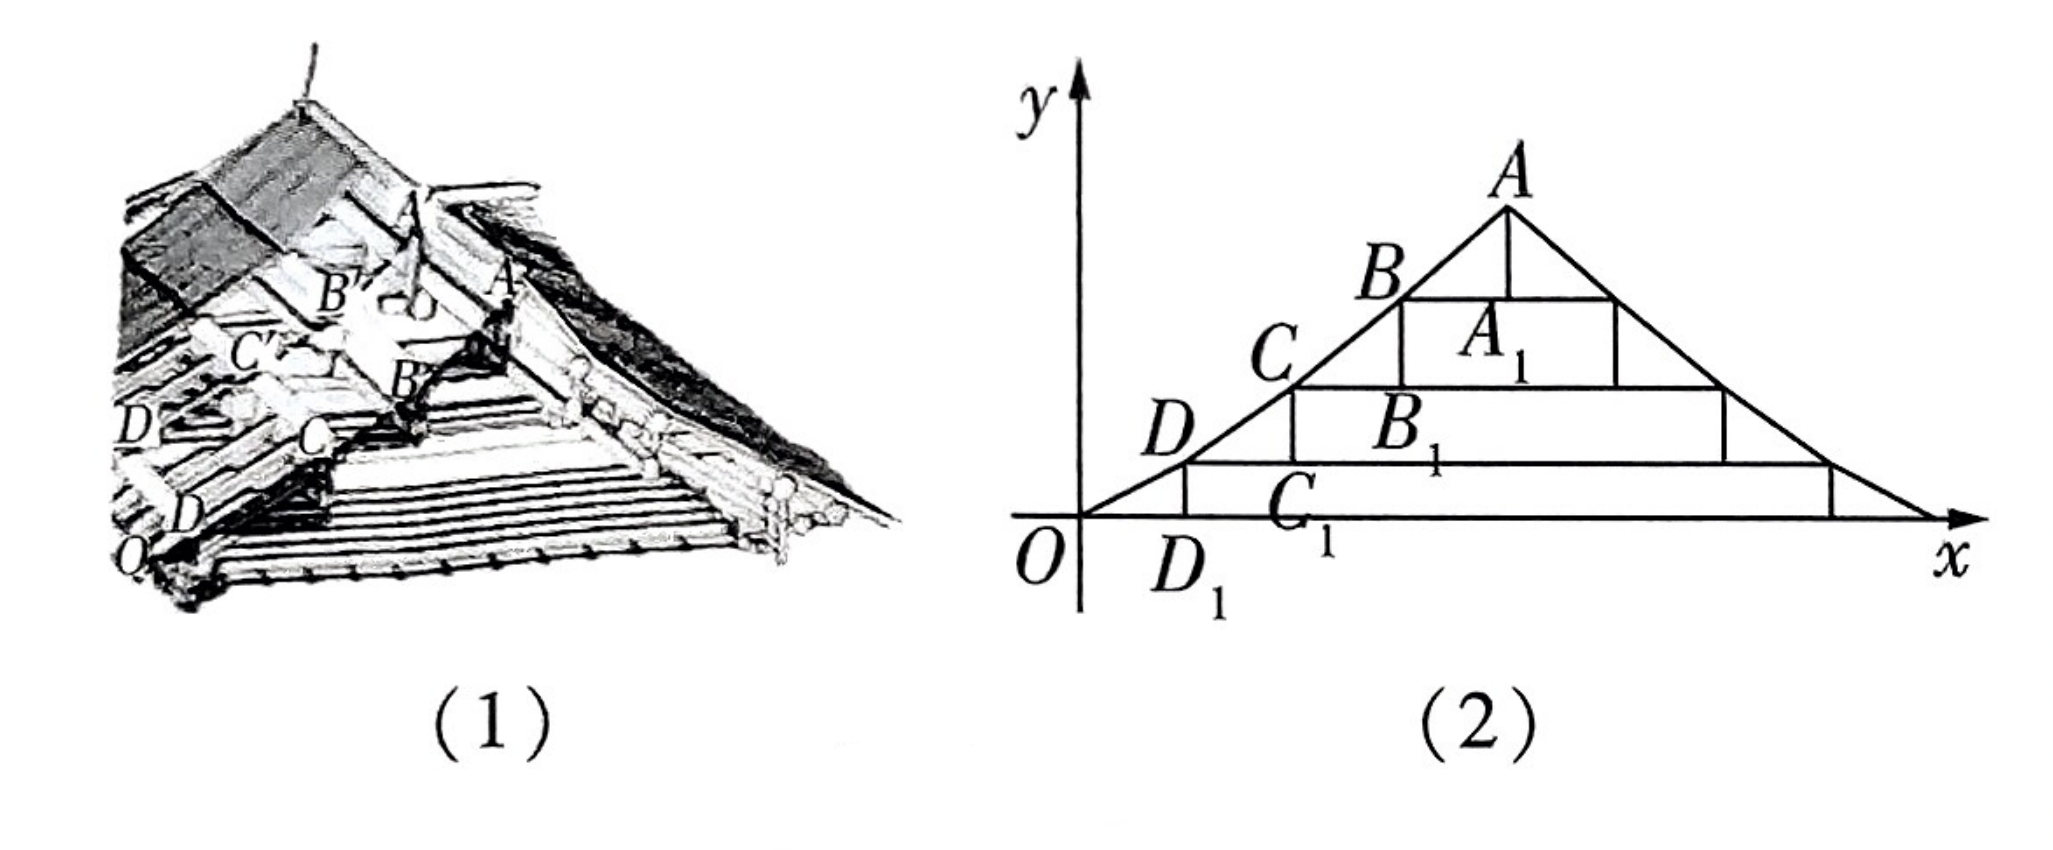
\includegraphics[width=0.8\textwidth]{2.png} % 不要加后缀 .jpg .png
\end{figure}

\noindent\textbf{例六： }（2023全国乙卷）记 \(S_n\) 为等差数列 \(\{a_n\}\) 的前 \(n\) 项和，已知 \(a_2 = 11\)，\(S_{10} = 40\)。
\begin{enumerate}
    \item 求 \(\{a_n\}\) 的通项公式；
    \item 求数列 \(\{|a_n|\}\) 的前 \(n\) 项和 \(T_n\)。
\end{enumerate}
\newpage

\noindent\textbf{例七： }（2023新高考一卷）设等差数列 \(\{a_n\}\) 的公差为 \(d\)，且 \(d > 1\)。令 \(b_n = \frac{n^2 + n}{a_n}\)，记 \(S_n, T_n\) 分别为数列 \(\{a_n\}, \{b_n\}\) 的前 \(n\) 项和。
\begin{enumerate}
    \item 若 \(3a_2 = 3a_1 + a_3\)，\(S_3 + T_3 = 21\)，求 \(\{a_n\}\) 的通项公式；
    \item 若 \(\{b_n\}\) 为等差数列，且 \(S_{99} - T_{99} = 99\)，求 \(d\)。
\end{enumerate}
\newpage

\subsection{等比数列}
\subsubsection{等比数列的的性质}
一般地，如果一个数列从第 2 项起，每一项与它的前一项的比都等于同一个常数，那么这个数列叫做\textcolor{cyan}{等比数列}（geometric progression），这个常数叫做等比数列的\textcolor{cyan}{公比}（common ratio），公比通常用字母 \(q\) 表示（显然 \(q \neq 0\)）。
定义还可以叙述为：在数列 \(\{a_n\}\) 中，若 \(\frac{a_{n+1}}{a_n} = q\)（\(q\) 为常数且 \(q \neq 0\)），则 \(\{a_n\}\) 是等比数列。
\vspace{2\baselineskip}


知识点 1. 形式：
\[
\begin{cases}
\text{通项} & a_n = a_1 q^{n-1} \quad (a_1, q \neq 0), \\
\text{通推} & a_{n+1} = q a_n, \\
\text{求和} & \text{见知识点 4}.
\end{cases}
\]
\vspace{1\baselineskip}

知识点 2. 等比中项：若 \(a, S, b\) 成等比数列，则 \(S = \sqrt{ab}\)，我们称 \(S\) 为 \(a, b\) 的等比中项（\(a, b\) 同号）。
\vspace{1\baselineskip}

知识点 3. 等比数列的单调性：

\begin{center}
\begin{tabular}{|>{\centering\arraybackslash}m{0.35\textwidth}|>{\centering\arraybackslash}m{0.55\textwidth}|}
\hline
条件 & 单调性 \\
\hline
\(\begin{cases} a_1 > 0, \\ q > 1 \end{cases}\) 或 \(\begin{cases} a_1 < 0, \\ 0 < q < 1 \end{cases}\) & \(\{a_n\}\) 为递增数列 \\
\hline
\(\begin{cases} a_1 > 0, \\ 0 < q < 1 \end{cases}\) 或 \(\begin{cases} a_1 < 0, \\ q > 1 \end{cases}\) & \(\{a_n\}\) 为递减数列 \\
\hline
\(q = 1\) & \(\{a_n\}\) 为常数列，不存在单调性 \\
\hline
\(q < 0\) & \(\{a_n\}\) 为摆动数列（所有奇数项同号，所有偶数项同号，但奇数项与偶数项异号），不存在单调性 \\
\hline
\end{tabular}
\end{center}

知识点 4. 等比数列的其他性质：
若数列 \(\{a_n\}\) 是公比为 \(q\) 的等比数列，则有如下性质：

\begin{enumerate}
    \item \(a_n = a_m q^{n-m}\ (m,n \in \mathbf{N}^*)\).

    \item 若 \(m+n=p+q\ (m,n,p,q \in \mathbf{N}^*)\)，则 \(a_m a_n = a_p a_q\)。
    \begin{enumerate}[label=\arabic*)]
        \item 特别地，若 \(m+n=2r\)，则 \(a_m a_n = a_r^2\ (m,n,r \in \mathbf{N}^*)\)；
        \item \(a_1 a_n = a_2 a_{n-1} = \dots = a_i a_{n+1-i}\ (n \in \mathbf{N}^*, n \geqslant 2, i = 1,2,\dots,n)\)。
    \end{enumerate}

    \item 若 \(m,n,p\ (m,n,p \in \mathbf{N}^*)\) 成等差数列，则 \(a_m,a_n,a_p\) 成等比数列。

    \item
    \begin{enumerate}[label=\arabic*)]
        \item 数列 \(\{\lambda a_n\}\)（\(\lambda\) 为不等于零的常数）仍是公比为 \(q\) 的等比数列；
        \item 数列 \(\left\{\frac{1}{a_n}\right\}\) 是公比为 \(\frac{1}{q}\) 的等比数列；
        \item 数列 \(\{|a_n|\}\) 是公比为 \(|q|\) 的等比数列；
        \item 若数列 \(\{b_n\}\) 是公比为 \(q'\) 的等比数列，则数列 \(\{a_n \cdot b_n\}\) 是公比为 \(q \cdot q'\) 的等比数列。
    \end{enumerate}

    \item 在数列 \(\{a_n\}\) 中，每隔 \(k(k \in \mathbf{N}^*)\) 项取出一项，按原来的顺序排列，所得数列仍为等比数列，且公比为 \(q^{k+1}\)。

    \item 在数列 \(\{a_n\}\) 中，依次每 \(k(k \in \mathbf{N}^*)\) 项的和（或积）构成公比为 \(q^k\)（或 \(q^{k^2}\)）的等比数列。

    \item
    \begin{enumerate}[label=\arabic*)]
        \item 已知 \(b>0\) 且 \(b \neq 1\)，如果数列 \(\{a_n\}\) 是以 \(d\) 为公差的等差数列，那么数列 \(\{b^{a_n}\}\) 是以 \(b^d\) 为公比的等比数列；
        \item 如果数列 \(\{a_n\}\) 是各项均为正且公比为 \(q\) 的等比数列，那么数列 \(\{\log_b a_n\}\) 是以 \(\log_b q\) 为公差的等差数列。
    \end{enumerate}
\end{enumerate}
\newpage

知识点5. 等比数列与指数函数的关系

等比数列 \(\{a_n\}\) 的通项公式 \(a_n = a_1 q^{n-1}\)，还可以整理为 \(a_n = \frac{a_1}{q} \cdot q^n\)，当 \(q > 0\) 且 \(q \neq 1\) 时，等比数列 \(\{a_n\}\) 的第 \(n\) 项 \(a_n\) 是函数 \(f(x) = \frac{a_1}{q} \cdot q^x\ (x \in \mathbf{R})\) 当 \(x = n\) 时的函数值，即 \(a_n = f(n)\)（如图 4.3.1-1 所示）。因此等比数列 \(\{a_n\}\) 的图象是函数 \(f(x) = \frac{a_1}{q} \cdot q^x\ (x \in \mathbf{R})\) 图象上的一些孤立的点。

\begin{figure}[H]
    \centering
    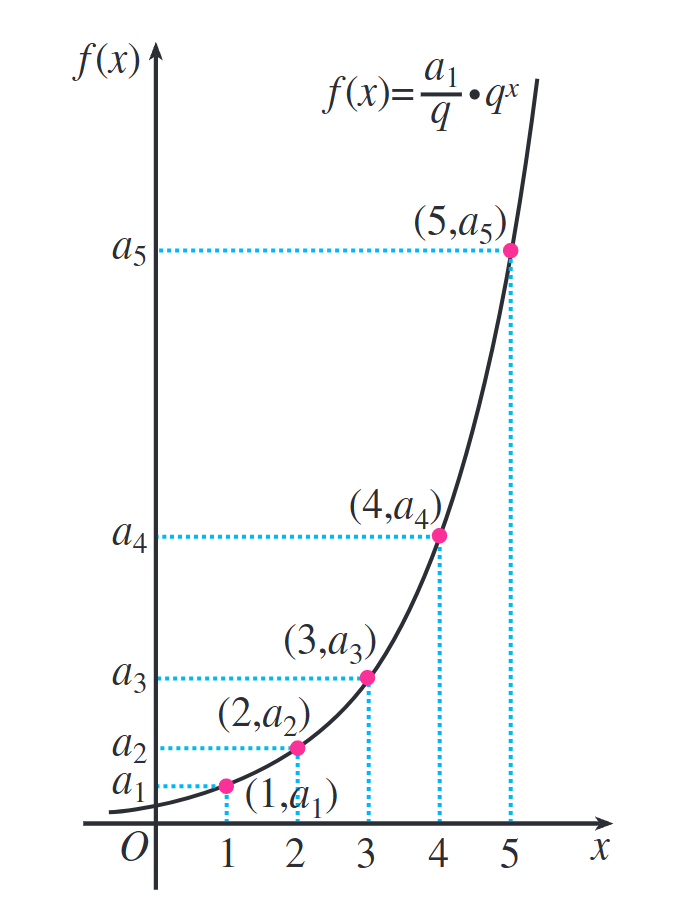
\includegraphics[width=0.4\textwidth]{3.png} % 不要加后缀 .jpg .png
\end{figure}

\begin{tcolorbox}[colback=blue!10,colframe=blue!70!black,title=]
    其实等差数列与等比数列亦有联系，如果我们对一个等比数列取对数（当然这个等比数列必须是正数数列），那么就会得到一个等差数列。
    事实上，利用对数进行加法和乘法之间的互相转化是一个很有效的数学工具。我们可以在多个数学板块中看到这一点，数列自然也不例外。
\end{tcolorbox}

\subsubsection{等比数列的求和}

等比数列的前$n$项和公式为：

\[
S_n =
\begin{cases}
\dfrac{a_1(1 - q^n)}{1 - q}, \;\;q\neq 1;\\[1em]
\dfrac{a_1 - a_n q}{1 - q},\;\;q\neq 1.
\end{cases}
\]

当$q=1$时，等比数列就成为了一个常数列，其前$n$项和为$a_1n$。

\begin{tcolorbox}[colback=blue!10,colframe=blue!70!black,title=]
    需要注意：常数列都是等差数列，非0的常数列都是等比数列，这一点经常用以举反例。
\end{tcolorbox}

这个公式的推导过程如下：

设等比数列 \(\{a_n\}\) 的首项为 \(a_1\)，公比为 \(q\)，则 \(\{a_n\}\) 的前 \(n\) 项和是
\[
S_n = a_1 + a_2 + a_3 + \dots + a_n.
\]

根据等比数列的通项公式，上式可写成
\[
S_n = a_1 + a_1 q + a_1 q^2 + \dots + a_1 q^{n-1}. \tag{1}
\]

如果用公比 \(q\) 乘①的两边，可得
\[
qS_n = a_1 q + a_1 q^2 + \dots + a_1 q^{n-1} + a_1 q^n. \tag{2}
\]

①②两式的右边有很多相同的项，用①的两边分别减去②的两边，就可以消去这些相同的项，可得
\[
S_n - qS_n = a_1 - a_1 q^n,
\]
即
\[
(1 - q)S_n = a_1(1 - q^n).
\]

整理后便可得到等比数列求和公式。在证明过程中用到的求和方法叫做错位相减法，这一方法我们会在后续的
讲义中细致讲解。
\vspace{1\baselineskip}
等比数列求和公式的性质：

1. 当 \(q = 1\) 时，\(\dfrac{S_n}{S_m} = \dfrac{n}{m}\)；当 \(q \neq \pm 1\) 时，\(\dfrac{S_n}{S_m} = \dfrac{1 - q^n}{1 - q^m}\)。
\vspace{1\baselineskip}

2. \(S_{n+m} = S_m + q^m S_n = S_n + q^n S_m\)。
\vspace{1\baselineskip}

3. 设 \(S_{\text{偶}}\) 与 \(S_{\text{奇}}\) 分别是偶数项的和与奇数项的和。
若项数为 \(2n\)，则 \(\dfrac{S_{\text{偶}}}{S_{\text{奇}}} = q\)；
若项数为 \(2n+1\)，则 \(\dfrac{S_{\text{奇}} - a_1}{S_{\text{偶}}} = q\)。
\vspace{1\baselineskip}

4. 当 \(q = -1\) 且 \(m\) 为奇数，或 \(q \neq -1\) 时，连续 \(m\) 项的和（如 \(S_m, S_{2m}-S_m, S_{3m}-S_{2m},\dots\)）仍组成等比数列，公比为 \(q^m\)（\(m \geqslant 2\)）。
\vspace{3\baselineskip}

\begin{center}
    小节练习
\end{center}

\noindent\textbf{例一： }（2023天津）已知 \(\{a_n\}\) 为等比数列，\(a_{n+1} = 2S_n + 2\)，则 \(a_4\) 的值为 \underline{\quad\quad}。
\vspace{2\baselineskip}

\noindent\textbf{例二： }已知各项均为正数的等比数列 \(\{a_n\}\) 满足：\(a_1 + a_2 + a_3 + a_4 = 15\) 且 \(a_5 = 3a_3 + 4a_1\)，则 \(a_3 = \underline{\quad\quad}\)。
\vspace{2\baselineskip}

\noindent\textbf{例三： }（2019天津）设 \(\{a_n\}\) 为等差数列，\(\{b_n\}\) 为等比数列，已知 \(a_1 = 4\)，\(b_1 = 6\)，\(b_2 = 2a_2 - 2\)，\(b_3 = 2a_3 + 4\)。则 \(\{a_n\}\) 与 \(\{b_n\}\) 的通项公式为？
\vspace{8\baselineskip}

\noindent\textbf{例四： } （课本原题）如图，正方形 \(ABCD\) 的边长为 \(5\ \mathrm{cm}\)，取正方形 \(ABCD\) 各边的中点 \(E\)，\(F\)，\(G\)，\(H\)，作第 2 个正方形 \(EFGH\)，然后再取正方形 \(EFGH\) 各边的中点 \(I\)，\(J\)，\(K\)，\(L\)，作第 3 个正方形 \(IJKL\)，依此方法一直继续下去。

(1) 求从正方形 \(ABCD\) 开始，连续 10 个正方形的面积之和；

(2) 如果这个作图过程可以一直继续下去，那么这些正方形的面积之和将趋近于多少？

\begin{figure}[H]
\centering
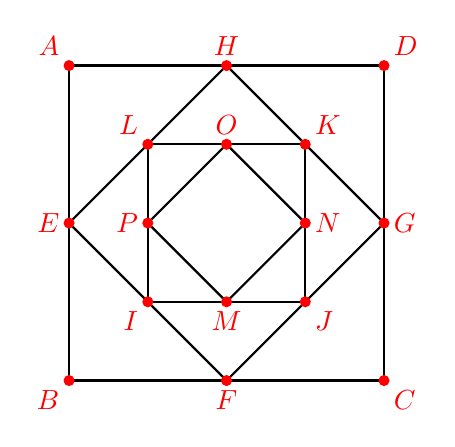
\begin{tikzpicture}[scale=1.0]
% 定义坐标
\coordinate (A) at (0,4);
\coordinate (B) at (0,0);
\coordinate (C) at (4,0);
\coordinate (D) at (4,4);
\coordinate (E) at (0,2);
\coordinate (F) at (2,0);
\coordinate (G) at (4,2);
\coordinate (H) at (2,4);
\coordinate (I) at (1,1);
\coordinate (J) at (3,1);
\coordinate (K) at (3,3);
\coordinate (L) at (1,3);
\coordinate (P) at (1,2);
\coordinate (N) at (3,2);
\coordinate (M) at (2,1);
\coordinate (O) at (2,3);

% 绘制最外层正方形 ABCD
\draw[thick] (A) -- (B) -- (C) -- (D) -- cycle;
% 绘制第2个正方形 EFGH
\draw[thick] (E) -- (F) -- (G) -- (H) -- cycle;
% 绘制第3个正方形 IJKL
\draw[thick] (I) -- (J) -- (K) -- (L) -- cycle;
% 绘制最内层小正方形
\draw[thick] (P) -- (M) -- (N) -- (O) -- cycle;

% 标记顶点
\fill[red] (A) circle (2pt) node[above left] {$A$};
\fill[red] (B) circle (2pt) node[below left] {$B$};
\fill[red] (C) circle (2pt) node[below right] {$C$};
\fill[red] (D) circle (2pt) node[above right] {$D$};
\fill[red] (E) circle (2pt) node[left] {$E$};
\fill[red] (F) circle (2pt) node[below] {$F$};
\fill[red] (G) circle (2pt) node[right] {$G$};
\fill[red] (H) circle (2pt) node[above] {$H$};
\fill[red] (I) circle (2pt) node[below left] {$I$};
\fill[red] (J) circle (2pt) node[below right] {$J$};
\fill[red] (K) circle (2pt) node[above right] {$K$};
\fill[red] (L) circle (2pt) node[above left] {$L$};
\fill[red] (P) circle (2pt) node[left] {$P$};
\fill[red] (N) circle (2pt) node[right] {$N$};
\fill[red] (M) circle (2pt) node[below] {$M$};
\fill[red] (O) circle (2pt) node[above] {$O$};
\end{tikzpicture}
\end{figure}

\newpage

\noindent\textbf{例五： }（2023全国甲卷）设等比数列 \(\{a_n\}\) 的各项均为正数，前 \(n\) 项和为 \(S_n\)，若 \(a_1 = 1\)，\(S_5 = 5S_3 - 4\)，
\vspace{1\baselineskip}

则 \(S_4 =\) \underline{\quad\quad}


\vspace{5\baselineskip}

\noindent\textbf{例六： }已知数列 \(\{a_n\}\) 的首项 \(a_1 = \frac{3}{5}\)，且满足 \(a_{n+1} = \frac{3a_n}{2a_n + 1}\)。

\begin{enumerate}
\item 求证：数列 \(\left\{\frac{1}{a_n} - 1\right\}\) 为等比数列。

\item 若 \(\frac{1}{a_1} + \frac{1}{a_2} + \frac{1}{a_3} + \dots + \frac{1}{a_n} < 100\)，求满足条件的最大整数 \(n\)。
\end{enumerate}
\vspace{15\baselineskip}

\noindent\textbf{例七： }已知数列 \(\{a_n\}\) 为等差数列，\(a_1 = 1\)，\(a_3 = 2\sqrt{2} + 1\)，前 \(n\) 项和为 \(S_n\)，数列 \(\{b_n\}\) 满足 \(b_n = \frac{S_n}{n}\)。

求证：
\begin{enumerate}
    \item 数列 \(\{b_n\}\) 为等差数列；
    \item 数列 \(\{a_n\}\) 中的任意三项均不能构成等比数列。
\end{enumerate}

\newpage

\section{题型专练}
\subsection{数列求和}
\subsubsection{错位相减}

错位相减：针对 \(\underbrace{(an+b)}_{\text{等差 } a_n} \cdot \underbrace{c q^{n-1}}_{\text{等比 } b_n}\) 型

步骤如下：

\begin{enumerate}
\item 列出和式：
\[
T_n = a_1 b_1 + a_2 b_2 + \cdots + a_n b_n
\]

\item 同乘公比：
\[
\begin{aligned}
q T_n &= a_1 b_1 q + a_2 b_2 q + \cdots + a_n b_n q \\
&= a_1 b_2 + a_2 b_3 + \cdots + a_n b_{n+1}
\end{aligned}
\]

\item 两式相减：
\[
\begin{aligned}
(1-q) T_n &= a_1 b_1 + (a_2 - a_1) b_2 + (a_3 - a_2) b_3 + \cdots + (a_n - a_{n-1}) b_n - a_n b_{n+1} \\
\Rightarrow (1-q) T_n &= a_1 b_1 + d(b_2 + b_3 + \cdots + b_n) - a_n b_{n+1} \\
&= a_1 b_1 + d \cdot \frac{b_2(1 - q^{n-1})}{1 - q} - a_n b_{n+1}\\
\Rightarrow T_n &= \frac{a_1 b_1 - a_n b_{n+1}}{1 - q}+d \cdot \frac{b_2(1 - q^{n-1})}{(1 - q)^2}
\end{aligned}
\]
\end{enumerate}
\vspace{2\baselineskip}

\noindent\textbf{例题： }求数列 \(a_n = (2n-1) \cdot 3^n\) 的前 \(n\) 项和
\vspace{10\baselineskip}

\noindent\textbf{例题： }求数列 \(b_n = (-1)^n \cdot n \cdot 2^{n+1}\) 的前 \(n\) 项和
\vspace{10\baselineskip}
\newpage

\subsubsection{并项求和}

并项求和：当需要我们进行求和的数列存在$(-1)^n$项时，我们当然可以将其拆分为两个数列分别求和，不过这样一般比较麻烦，因此我们可以
考虑并项求和，即先将相邻的两项加起来在总体求和，倘若我们从第一项开始，即第一项搭配第二项、第三项搭配第四项……，那么我们就不需要再讨论$(-1)^2$
的正负情况了，因为我们的每一个“小单元”都是先奇后偶，先负后正。这种方法特别适用于题干中让我们求2n项的和时，因为这样我们就可以完美地进行并项求和。
当然，如果题干中出现类似这样$cos(\frac{2n\pi}{3})$的项，我们也可以考虑并项求和，因为$cos(\frac{2n\pi}{3}) $以3为周期，因此我们可以进行并三项求和，
当然我们也可以将其分为三个数列分别求和，具体哪种情况好用需要根据具体数列的形式分析。
\vspace{2\baselineskip}

\noindent \textbf{例题： } （2022天津)设$\{a_n\}$是等差数列，$\{b_n\}$是等比数列，且$a_1 = b_1 = a_2 - b_2 = a_3 - b_3 = 1$.

\begin{enumerate}
    \item 求$\{a_n\}$与$\{b_n\}$的通项公式；
    \item 设$\{a_n\}$的前$n$项和为$S_n$，求证：$(S_{n+1} + a_{n+1})b_n = S_{n+1}b_{n+1} - S_nb_n$；
    \item 求$\sum_{k=1}^{2n}\bigl[a_{k+1} - (-1)^k a_k\bigr]b_k$.
\end{enumerate}

\newpage

\subsubsection{分组求和}

分组求和：当数列的奇数项和偶数项遵循不一样的规律的时候，我们通常需要将它们分为两个子数列，然后分别求和再相加。
当然，我们也可以按照具体题目将数列分为三个或多个子数列的加和。
\vspace{2\baselineskip}

\noindent \textbf{例题： } (2024福建省厦门市四检) 设 \(S_n\) 为数列 \(\{a_n\}\) 的前 \(n\) 项和，已知 \(a_1 = 1\)，\(S_4 = 10\)，且 \(\left\{\frac{S_n}{n}\right\}\) 为等差数列.

\begin{enumerate}
    \item 求 \(\{a_n\}\) 的通项公式；
    \item 若 \(b_n = \begin{cases}
    a_n, & n \text{ 为奇数}, \\
    \dfrac{1}{a_n a_{n+2}}, & n \text{ 为偶数},
    \end{cases}\) 求 \(\{b_n\}\) 的前 \(2n\) 项和 \(T_{2n}\).
\end{enumerate}


\newpage


\subsubsection{裂项相消}

裂项相消：就是把一个一个数列$a_n$中的每一项拆分为$a_n=b_{n+1}-b_n$这样就有：

$$S_n=\sum_{k=1}^n a_k=\sum_{k=1}^n (b_{k+1}-b_k)=(b_{n+1}-b_n)+(b_n-b_{n-1})+\cdots+(b_2-b_1)+b_1=b_{n+1}-b_1$$
\vspace{1\baselineskip}

裂项相消有不同的类别：
\vspace{1\baselineskip}

$\diamondsuit$ 基础型：
\vspace{1\baselineskip}

\begin{align}
\frac{1}{n(n+1)} &= \frac{1}{n} - \frac{1}{n+1}, \label{eq:split1} \\
\frac{1}{n(n+t)} &= \frac{1}{t}\left( \frac{1}{n} - \frac{1}{n+t} \right) \quad (t \neq 0). \label{eq:split3}\\
\frac{1}{a_n a_{n+1}} &= \frac{1}{d}\left( \frac{1}{a_n} - \frac{1}{a_{n+1}} \right).
\end{align}

$\text{其中}\ \{a_n\}\ \text{为等差数列}, d\ \text{为公差}, \ a_n \neq 0\ \text{且}\ d \neq 0$，事实上我们看到公式(1)(2)是公式(3)的特殊情况

\begin{align}
\frac{1}{\sqrt{n+1}+\sqrt{n}} &= \sqrt{n+1} - \sqrt{n},
\end{align}



$\diamondsuit$ 指数型：
\vspace{1\baselineskip}

对于含有指数的通项，该如何裂项呢？

例如：
\[
\frac{2^{n+1}}{(2^{n+1}+1)(2^n+1)},\quad \frac{n\cdot 2^{n+1}}{(n+1)(n+2)}
\]

一般通过两步解决：1.分解分母猜分母；2.分子设参求分子。

例如：\(\displaystyle \frac{2^{n+1}}{(2^{n+1}+1)(2^n+1)}\)，通过其分母的形式，我们猜想其分解后应形如：
\[
\frac{?}{2^n+1} - \frac{?}{2^{n+1}+1}.
\]

接下来，我们考虑分子的形式，通过分解前的分子 \(2^{n+1}\) 可以猜出：分子应当不含幂次项或 \(n^2\) 项（以及 \(n\) 的更高次），于是我们可以分别设 \(?\) 处为 \(an+b\)、\(a(n+1)+b\)（这是因为要想做到裂项，减号左右必须是$a_n$与$a_{n-1}$的关系）然后解出系数。
当然我们还有更简便的方法，就是直接把两个分子设为A和B，然后将n视为一个常数来求解AB，最后AB就可以写为关于n的表达式，当然这样并不能确保裂项成功，因为我们的假设中没有任何对AB的约束，然而事实上它们有很强的关系。
下面的例一用的是简便的方法，例题二用的是需要预先猜出分子大致结构的方法。


\subsection*{例1：拆分 \(\displaystyle \frac{2^{n+1}}{(2^{n+1}+1)(2^n+1)}\)}
设裂项形式为：
\begin{align*}
\frac{2^{n+1}}{(2^{n+1}+1)(2^n+1)} &= \frac{A}{2^n+1} - \frac{B}{2^{n+1}+1},
\end{align*}
通分后分子相等：
\begin{align*}
2^{n+1} &= A(2^{n+1}+1) - B(2^n+1) \\
2^{n+1} &= (2A - B)2^n + (A - B).
\end{align*}
比较两边系数得方程组：
\[
\begin{cases}
2A - B = 2, \\
A - B = 0.
\end{cases}
\]
解得 \(A = B = 2\)，因此裂项结果为：
\begin{align*}
\frac{2^{n+1}}{(2^{n+1}+1)(2^n+1)} &= \frac{2}{2^n+1} - \frac{2}{2^{n+1}+1}.
\end{align*}

\subsection*{例2：拆分 \(\displaystyle \frac{n\cdot 2^{n+1}}{(n+1)(n+2)}\)}
先拆分分式结构，设裂项形式为：
\begin{align*}
\frac{n\cdot 2^{n+1}}{(n+1)(n+2)} &= \frac{A\cdot 2^n}{n+1} - \frac{B\cdot 2^n}{n+2},
\end{align*}
通分后分子相等：
\begin{align*}
n\cdot 2^{n+1} &= A\cdot 2^n (n+2) - B\cdot 2^n (n+1) \\
2n &= A(n+2) - B(n+1) \\
2n &= (A - B)n + (2A - B).
\end{align*}
比较两边系数得方程组：
\[
\begin{cases}
A - B = 2, \\
2A - B = 0.
\end{cases}
\]
解得 \(A = -2\)，\(B = -4\)，代入后裂项结果为：
\begin{align*}
\frac{n\cdot 2^{n+1}}{(n+1)(n+2)} &= \frac{-2\cdot 2^n}{n+1} - \frac{-4\cdot 2^n}{n+2} \\
&= \frac{2^{n+2}}{n+2} - \frac{2^{n+1}}{n+1}.
\end{align*}
有了通用的方法，下面这些公式就交由读者补全：

\begin{align*}
\frac{n+2}{n(n+1)2^{n+1}} &= \;\;\;\;\;\;\;\;\;\;\;\;\;\;\;\;\;\;\;\; \;\;\;\;\;\;\;\;\;\;\;\;\;\;\;\;\;\;\;\;\\
\frac{3^n}{(3^n - 1)(3^{n+1} - 1)} &=   \\
\frac{(2n-1)3^n}{n(n+1)} &= 
\end{align*}

$\diamondsuit$ 有理函数型:
\vspace{1\baselineskip}

\begin{tcolorbox}[colback=blue!10,colframe=blue!70!black,title=]
有理函数就是分子分母均为多项式的函数,我们在函数板块也多次处理这类函数，一般来说，处理这种函数的第一步就是通过分离常数，使得分子次数严格小于分母次数。
\end{tcolorbox}

下面三个公式无需记忆（读者可以看到这些公式并没有标号）
\begin{align*}
\frac{1}{n(n+1)(n+2)} &= \frac{1}{2}\left( \frac{1}{n(n+1)} - \frac{1}{(n+1)(n+2)} \right), \\
\frac{n+1}{n^2(n+2)^2} &= \frac{1}{4}\left( \frac{1}{n^2} - \frac{1}{(n+2)^2} \right), \\
\frac{(2n)^2}{(2n-1)(2n+1)} &= 1 + \frac{1}{2}\left( \frac{1}{(2n-1)} - \frac{1}{(2n+1)} \right).
\end{align*}
\newpage

我们解决这类数列的裂项问题和刚才所讲的指数型是高度一致的，具体步骤如下：

\begin{enumerate}
\item 分离常数，使分子的次数严格小于分母的次数。
\item 将分离后的两个分子设出来，由于此时分子的次数依然不可能大于或等于分母的次数，因此我们可以设出分子的更具体的形式，倘若分母是二次，那么我们就可以把两个分子分别设成$an+b$和$a(n+1)+b$
\end{enumerate}

请读者补全下列公式：

\begin{align*}
\frac{2n+1}{n^2(n+1)^2} &=  \;\;\;\;\;\;\;\; \;\;\;\;\;\;\;\; \;\;\;\;\;\;\;\; \;\;\;\;\;\;\ \;\;\;\;\;\;\\\
\frac{n+1}{n+2} + \frac{n+2}{n+1} &= 
\end{align*}



$\diamondsuit$ 裂项相“加”型:
\vspace{1\baselineskip}
裂项相消，即是构造相减的形式，而如果目标函数的结构是${(-1)^na_n}$,那么我们就要进行裂项相加：$(-1)^na_n=(-1)^n(b_{n+1}+b_n)$，这样就有：

\begin{align*}
S_n=\sum_{n=1}^n (-1)^na_n &=\sum_{n=1}^n (-1)^n(b_{n+1}+b_n) \\
&=-(b_2+b_1)+(b_3+b_2)-(b_4+b_3)+\cdots+(-1)^n(b_{n+1}+b_n) \\
&=-b_1+(-1)^nb_{n+1}
\end{align*}
 
\begin{tcolorbox}[colback=blue!10,colframe=blue!70!black,title=]
在进行裂项相消时，我们需要留意前后各有那些项被留了下来。一个非常简便的方法是：看前面留下了哪些项，后面就会对称留下哪些项，例如在上面的裂项中，
正数第二项$b_1$被留下，那么相应的倒数第二项也会被留下。
\end{tcolorbox}

于是我们有：

\begin{align*}
(-1)^{n-1} \frac{4n}{(2n-1)(2n+1)} &= (-1)^{n-1}\left( \frac{1}{2n-1} + \frac{1}{2n+1} \right), \\
(-1)^n \frac{2n+1}{n(n+1)} &= (-1)^n\left( \frac{1}{n} + \frac{1}{n+1} \right), \\
(-1)^{n+1} \frac{n+1}{(2n+1)(2n+3)} &= \frac{1}{4} \cdot (-1)^{n+1}\left( \frac{1}{2n+1} + \frac{1}{2n+3} \right), \\
(-1)^n \frac{6n-5}{(3n-4)(3n-1)} &= (-1)^n\left( \frac{1}{3n-4} + \frac{1}{3n-1} \right), \\
(-1)^n \frac{1}{\sqrt{n+1}-\sqrt{n}} &= (-1)^n\left( \sqrt{n+1} + \sqrt{n} \right), \\
(-1)^n \log(n^2 + n) &= (-1)^n\bigl[\log n + \log(n+1)\bigr].
\end{align*}

此处log的意思是，此对数的底数并不重要，无论以何数为底，结果都是相同的。

\newpage

$\diamondsuit$ 三角函数型*:
\vspace{1\baselineskip}

\begin{tcolorbox}[colback=blue!10,colframe=blue!70!black,title=]
\subsection*{和差化积公式}
\begin{align*}
\sin \alpha + \sin \beta &= 2\sin\frac{\alpha+\beta}{2}\cos\frac{\alpha-\beta}{2}, \\
\sin \alpha - \sin \beta &= 2\cos\frac{\alpha+\beta}{2}\sin\frac{\alpha-\beta}{2}, \\
\cos \alpha + \cos \beta &= 2\cos\frac{\alpha+\beta}{2}\cos\frac{\alpha-\beta}{2}, \\
\cos \alpha - \cos \beta &= -2\sin\frac{\alpha+\beta}{2}\sin\frac{\alpha-\beta}{2}.
\end{align*}

\subsection*{积化和差公式}
\begin{align*}
\sin \alpha \cos \beta &= \frac{1}{2}\bigl[\sin(\alpha+\beta) + \sin(\alpha-\beta)\bigr], \\
\cos \alpha \sin \beta &= \frac{1}{2}\bigl[\sin(\alpha+\beta) - \sin(\alpha-\beta)\bigr], \\
\cos \alpha \cos \beta &= \frac{1}{2}\bigl[\cos(\alpha+\beta) + \cos(\alpha-\beta)\bigr], \\
\sin \alpha \sin \beta &= -\frac{1}{2}\bigl[\cos(\alpha+\beta) - \cos(\alpha-\beta)\bigr].
\end{align*}
\end{tcolorbox}

\begin{align}
\tan(n+1)\tan n &= \frac{\tan(n+1)-\tan n}{\tan 1} - 1,\\
\frac{1}{\cos n \cos(n-1)} &= \frac{\tan n - \tan(n-1)}{\sin 1}\\
\frac{1}{\sin(n+1) \sin n} &= \frac{1}{\sin 1}\left( \frac{1}{\tan n} -\frac{1}{\tan(n+1)}\right)
\end{align}

上述公式(6)(7)的证明核心是将$\sin 1$拆成$sin((n+1)-n)$.下面我们来看一个稍有难道的例题，用来说明裂项相消的思路在三角函数的计算中亦有其应用。
\vspace{1\baselineskip}

事实上，上面的几个公式不过是一些特殊情况，更一般的，我们有：

\begin{align*}
\tan a_n \cdot \tan a_{n+1} &= \frac{\tan a_n - \tan a_{n+1}}{\tan d} - 1; \\
\frac{1}{\cos a_n \cdot \cos a_{n+1}} &= \frac{\tan a_{n+1} - \tan a_n}{\sin d}; \\
\frac{1}{\sin a_n \cdot \sin a_{n+1}} &= \frac{\cot a_{n+1} - \cot a_n}{\sin d}; \\
\cos a_n &= \frac{\sin\!\left(a_n + \frac{d}{2}\right) - \sin\!\left(a_n - \frac{d}{2}\right)}{2\sin\frac{d}{2}}; \\
\sin a_n &= -\frac{\cos\!\left(a_n + \frac{d}{2}\right) - \cos\!\left(a_n - \frac{d}{2}\right)}{2\sin\frac{d}{2}}.
\end{align*}

其中$a_n$是公差为d的等差数列。
\newpage

\noindent\textbf{例题： } 求下式的值：

\[
\cos\frac{\pi}{13}+\cos\frac{3\pi}{13}+\cos\frac{5\pi}{13}+\cos\frac{7\pi}{13}+\cos\frac{9\pi}{13}+\cos\frac{11\pi}{13}.
\]
\vspace{1\baselineskip}

\noindent\textbf{分析： } 

反复利用积化和差与和差化积公式计算原式，当项数较多时，其方法有两种：配对或裂项，本题采用裂项方法。

\noindent\textbf{解： }
\begin{align*}
&\cos\frac{\pi}{13}+\cos\frac{3\pi}{13}+\cos\frac{5\pi}{13}+\cos\frac{7\pi}{13}+\cos\frac{9\pi}{13}+\cos\frac{11\pi}{13} \\
&= \frac{1}{2\sin\frac{\pi}{13}}\Bigl(2\sin\frac{\pi}{13}\cos\frac{\pi}{13}+2\sin\frac{\pi}{13}\cos\frac{3\pi}{13}+2\sin\frac{\pi}{13}\cos\frac{5\pi}{13} \\
&\quad +2\sin\frac{\pi}{13}\cos\frac{7\pi}{13}+2\sin\frac{\pi}{13}\cos\frac{9\pi}{13}+2\sin\frac{\pi}{13}\cos\frac{11\pi}{13}\Bigr) \\
&= \frac{1}{2\sin\frac{\pi}{13}}\Bigl[\sin\frac{2\pi}{13}+\Bigl(\sin\frac{4\pi}{13}-\sin\frac{2\pi}{13}\Bigr)+\Bigl(\sin\frac{6\pi}{13}-\sin\frac{4\pi}{13}\Bigr) \\
&\quad +\Bigl(\sin\frac{8\pi}{13}-\sin\frac{6\pi}{13}\Bigr)+\Bigl(\sin\frac{10\pi}{13}-\sin\frac{8\pi}{13}\Bigr)+\Bigl(\sin\frac{12\pi}{13}-\sin\frac{10\pi}{13}\Bigr)\Bigr] \\
&= \frac{1}{2\sin\frac{\pi}{13}}\cdot\sin\frac{12\pi}{13} \\
&= \frac{1}{2}.
\end{align*}

\noindent\textbf{评注： } 
由本题的结论，再结合算式 $\cos\frac{\pi}{3},\ \cos\frac{\pi}{5}+\cos\frac{3\pi}{5},\ \cos\frac{\pi}{7}+\cos\frac{3\pi}{7}+\cos\frac{5\pi}{7},\ \cos\frac{\pi}{9}+\cos\frac{3\pi}{9}+\cos\frac{5\pi}{9}+\cos\frac{7\pi}{9}$ 的值，我们可以归纳猜想：
\[
\cos\frac{\pi}{2n+1}+\cos\frac{3\pi}{2n+1}+\cos\frac{5\pi}{2n+1}+\cdots+\cos\frac{2n-1}{2n+1}\pi=\frac{1}{2}.
\]

\noindent\textbf{证明} 令
\[
S = \cos\frac{\pi}{2n+1}+\cos\frac{3\pi}{2n+1}+\cos\frac{5\pi}{2n+1}+\cdots+\cos\frac{2n-1}{2n+1}\pi,
\]
则
\begin{align*}
2\sin\frac{\pi}{2n+1}\cdot S &= \sin\frac{2\pi}{2n+1}+\Bigl(\sin\frac{4\pi}{2n+1}-\sin\frac{2\pi}{2n+1}\Bigr) \\
&\quad +\Bigl(\sin\frac{6\pi}{2n+1}-\sin\frac{4\pi}{2n+1}\Bigr)+\cdots \\
&\quad +\Bigl(\sin\frac{2n}{2n+1}\pi-\sin\frac{2n-2}{2n+1}\pi\Bigr) \\
&= \sin\frac{2n}{2n+1}\pi.
\end{align*}
于是
\[
S = \frac{1}{2}.
\]

下面我们来证明一个三角函数恒等式：
\[
S_n = \cos x + \cos 2x + \cos 3x + \dots + \cos nx=\frac{\cos\left(\frac{n+1}{2}x\right)\sin\left(\frac{nx}{2}\right)}{\sin\frac{x}{2}}.
\]
给等式两边同乘 $2\sin\frac{x}{2}$：
\begin{align*}
2\sin\frac{x}{2} \cdot S_n &= 2\sin\frac{x}{2}\cos x + 2\sin\frac{x}{2}\cos 2x + 2\sin\frac{x}{2}\cos 3x + \dots + 2\sin\frac{x}{2}\cos nx.
\end{align*}
根据**积化和差公式**：$2\sin A \cos B = \sin(A+B) - \sin(A-B)$，对每一项展开：
\begin{align*}
2\sin\frac{x}{2}\cos kx &= \sin\left(\frac{x}{2} + kx\right) - \sin\left(\frac{x}{2} - kx\right) \\
&= \sin\left(\frac{2k+1}{2}x\right) - \sin\left(\frac{1-2k}{2}x\right) \\
&= \sin\left(kx + \frac{x}{2}\right) + \sin\left(kx - \frac{x}{2}\right).
\end{align*}
将展开式代入求和式，逐项裂项：
\begin{align*}
2\sin\frac{x}{2} \cdot S_n &= \left(\sin\frac{3x}{2} - \sin\frac{x}{2}\right) + \left(\sin\frac{5x}{2} - \sin\frac{3x}{2}\right) + \left(\sin\frac{7x}{2} - \sin\frac{5x}{2}\right) + \dots + \left(\sin\left(nx + \frac{x}{2}\right) - \sin\left(nx - \frac{x}{2}\right)\right).
\end{align*}
裂项后中间项全部抵消，仅剩首尾项：
\begin{align*}
2\sin\frac{x}{2} \cdot S_n &= \sin\left(nx + \frac{x}{2}\right) - \sin\frac{x}{2}.
\end{align*}
对右边再次使用和差化积公式：$\sin A - \sin B = 2\cos\frac{A+B}{2}\sin\frac{A-B}{2}$，化简：
\begin{align*}
\sin\left(\frac{2n+1}{2}x\right) - \sin\frac{x}{2} &= 2\cos\left(\frac{\frac{2n+1}{2}x + \frac{x}{2}}{2}\right)\sin\left(\frac{\frac{2n+1}{2}x - \frac{x}{2}}{2}\right) \\
&= 2\cos\left(\frac{n+1}{2}x\right)\sin\left(\frac{nx}{2}\right).
\end{align*}
将化简结果代回，两边同除以 $2\sin\frac{x}{2}$（需满足 $\sin\frac{x}{2} \neq 0$，即 $x \neq 2k\pi, k\in\mathbb{Z}$）：
\begin{align*}
S_n &= \frac{\cos\left(\frac{n+1}{2}x\right)\sin\left(\frac{nx}{2}\right)}{\sin\frac{x}{2}}.
\end{align*}


$\diamondsuit$ 对数型*:
\vspace{1\baselineskip}

事实上，这种裂项方式并没有什么特殊，关键还是在于先猜出裂项后的分母，再通过待定系数法等操作求出分子，我们仅举一例对此进行说明。
\vspace{1\baselineskip}

\noindent\textbf{例题： } 
若数列$\{b_n\}$满足，

\large 
\[
b_n=e^{\frac{[(2n-1)+\ln n (n-1)]\ln b_{n-1}}{(2n-1)+\ln n (n-1)+[ln(n-1)^{n-1}-ln n^n]ln b_{n-1}}} \;\;\;\;(n\ge 2)
\]
\normalsize

且$b_1=e$。

\noindent\textbf 1.求数列$\{b_n\}$的通项公式；

\noindent\textbf 2.求数列$\{b_n\}$的前$n$项和$S_n$。


\noindent\textbf{解：}

当$n\ge 2$时，对原式两边同时取对数得：

\[
\ln b_n = \frac{[(2n-1)+\ln n (n-1)]\ln b_{n-1}}{(2n-1)+\ln n (n-1)+[ln(n-1)^{n-1}-ln n^n]ln b_{n-1}}
\]
将上式分子分母倒过来：
\[
\frac{1}{\ln b_n} = \frac{(2n-1)+\ln n (n-1)+[ln(n-1)^{n-1}-ln n^n]ln b_{n-1}}{[(2n-1)+\ln n (n-1)]\ln b_{n-1}} = \frac{1}{ln b_{n-1}}+\frac{\ln(n-1)^{n-1}-\ln n^n }{(2n-1)+\ln n (n-1)}.
\]
裂项可得：
\[
\frac{1}{\ln b_n} - \frac{1}{\ln b_{n+1}} = \frac{1}{n+\ln n} - \frac{1}{(n-1)+\ln(n-1)}.
\]
于是
\[
\begin{cases}
\frac{1}{\ln b_n} - \frac{1}{\ln b_{n-1}} = \frac{1}{n+\ln n} - \frac{1}{(n-1)+\ln(n-1)}, \\
\frac{1}{\ln b_{n-1}} - \frac{1}{\ln b_{n-2}} = \frac{1}{(n-1)+\ln(n-1)} - \frac{1}{(n-2)+\ln(n-2)}, \\
\cdots\cdots \\
\frac{1}{\ln b_3} - \frac{1}{\ln b_2} = \frac{1}{2+\ln 2} - \frac{1}{1+\ln 1}, \\
\frac{1}{\ln b_2} = 1.
\end{cases}
\]
累加得
\[
\frac{1}{\ln b_n} = \frac{1}{n+\ln n} \implies \ln b_n = \ln n \cdot e^n \implies b_n = n \cdot e^n.
\]

使用错位相减法：
\[
eS_n = 1\cdot e^2 + 2\cdot e^3 + \cdots + (n-1)\cdot e^n + n\cdot e^{n+1},
\]
\[
\Rightarrow (1-e)S_n = e + e^2 + e^3 + \cdots + e^n - n\cdot e^{n+1} = \frac{e-e^{n+1}}{1-e} - n\cdot e^{n+1},
\]
\[
\Rightarrow S_n = \frac{e-e^{n+1}}{(1-e)^2} - \frac{n\cdot e^{n+1}}{1-e}.
\]
\vspace{1\baselineskip}


$\diamondsuit$ 某些特殊裂项*:
\vspace{1\baselineskip}

\begin{align}
    \frac{n}{(n+1)!}&=\frac{1}{n!} - \frac{1}{(n+1)!}\\
    n(n+1)!&=(n+1)!-n!\\
    n(n+1)&=\frac{1}{3}[n(n+1)(n+2)-(n-1)n(n+1)]
\end{align}

\begin{tcolorbox}[colback=blue!10,colframe=blue!70!black,title=]
    读者可以尝试用公式(10)来证明一个很重要的求和公式，尽管这个公式并非课内要求，但它出现的频率是很高的（至少在高考物理中出现的频率是很高的）
    $$1^2+2^2+3^2+\cdots+n^2=\frac{n(n+1)(2n+1)}{6}$$
\end{tcolorbox}

\noindent\textbf{例题: }(2020天津)已知$\{a_n\}$为等差数列，$\{b_n\}$为等比数列，且满足

\[
a_1 = b_1 = 1,\quad a_5 = 5(a_4 - a_3),\quad b_5 = 4(b_4 - b_3).
\]

\noindent 1.求$\{a_n\}$和$\{b_n\}$的通项公式；

\noindent 2.记$\{a_n\}$的前$n$项和为$S_n$，求证：$S_n S_{n+2} < S_{n+1}^2\ (n\in\mathbf{N}^*)$；

\noindent 3.对任意的正整数$n$，设
\[
c_n =
\begin{cases}
\dfrac{(3a_n - 2)b_n}{a_n a_{n+2}}, & n\text{为奇数}, \\[6pt]
\dfrac{a_{n-1}}{b_{n+1}}, & n\text{为偶数}.
\end{cases}
\]
求数列$\{c_n\}$的前$2n$项和。
\newpage

\subsubsection{倒序相加}

当一个数列第一项和最后一项，第二项和倒数第二项，……可以很容易的相加，并且相加后的结果是易于求和的，那么我们就看如下操作：

\begin{align*}
    S_n&=a_1+a_2+\cdots +a_n\\
    S_n&=a_n+a_{n-1}\cdots +a_1
\end{align*}

两式相加得：

$$2S_n=(a_1+a_n)+(a_2+a_{n-1})+\cdots+(a_n+a_1)$$

然后继续求和
\vspace{1\baselineskip}

\noindent\textbf{例题： （2024河西区三模）已知递增数列$\{a_n\}$的前$n$项和为$S_n$，且$4S_n = a_n^2 + 4n$，$n\in\mathbf{N}^*$。}

\begin{enumerate}[label=(\Roman*)] % 第一层编号：(I)(II)(III)...
    \item 求数列$\{a_n\}$的通项公式；
    
    \item 设$b_n = a_1 \mathrm{C}_n^1 + a_2 \mathrm{C}_n^2 + a_3 \mathrm{C}_n^3 + \dots + a_n \mathrm{C}_n^n$。
    \begin{enumerate}[label=(\roman*)] % 第二层编号：(ⅰ)(ⅱ)(ⅲ)...
        \item 求数列$\{b_n\}$的通项公式；
        \item 求$\displaystyle\sum_{i=1}^n \left( \frac{12b_i - 2^{i+3}}{a_i \cdot a_{i+2}} \right)$。
    \end{enumerate}
\end{enumerate}
\newpage

\begin{center}
    小节练习
\end{center}


\noindent\textbf{例一： }（2019天津）
设$\{a_n\}$是等差数列，$\{b_n\}$是等比数列。已知$a_1=4$，$b_1=6$，$b_2=2a_2-2$，$b_3=2a_3+4$。

\begin{enumerate}[label=(\Roman*)]
    \item 求$\{a_n\}$和$\{b_n\}$的通项公式；
    
    \item 设数列$\{c_n\}$满足$c_1=1$，
    \[
    c_n =
    \begin{cases}
    1, & 2^k < n < 2^{k+1}, \\
    b_k, & n = 2^k,
    \end{cases}
    \]
    其中$k\in\mathbf{N}^*$。
    
    \begin{enumerate}[label=(\roman*)]
        \item 求数列$\{a_{2^n}(c_{2^n}-1)\}$的通项公式；
        \item 求$\displaystyle\sum_{i=1}^{2^n} a_i c_i\ (n\in\mathbf{N}^*)$。
    \end{enumerate}
\end{enumerate}
\vspace{15\baselineskip}

\noindent\textbf{例二： （2024天津）已知数列$\{a_n\}$是公比大于 0 的等比数列，其前$n$项和为$S_n$。若$a_1=1$，$S_2=a_3-1$。}

\begin{enumerate}[label=(\Roman*)]
    \item 求数列$\{a_n\}$前$n$项和$S_n$；
    
    \item 设$b_n =
    \begin{cases}
    k, & n = a_k, \\
    b_{n-1} + 2k, & a_k < n < a_{k+1},
    \end{cases}$
    $b_1=1$，其中$k$是大于 1 的正整数。
    
    \begin{enumerate}[label=(\roman*)]
        \item 当$n = a_{k+1}$时，求证：$b_{n-1} \ge a_k \cdot b_n$；
        \item 求$\displaystyle\sum_{i=1}^{S_n} b_i$。
    \end{enumerate}
\end{enumerate}

\newpage

\noindent\textbf{例三： }（2024红桥二模）已知$\{a_n\}$是等差数列，$\{b_n\}$是公比为正数的等比数列，且$b_1=1$，$b_2+2b_3=1$，$(a_2+a_6)b_4=1$，$a_4b_2=a_5-a_3$。

\begin{enumerate}[label=(\Roman*)]
    \item 求数列$\{a_n\},\{b_n\}$的通项公式；
    
    \item 设$c_n=1+\dfrac{1}{a_n(a_n+2)}$，$S_n=c_1 \cdot c_2 \cdot c_3 \cdot \cdots \cdot c_n\ (n\in\mathbf{N}^*)$。
    
    \begin{enumerate}[label=(\roman*)]
        \item 求$S_n$；
        \item 求$\displaystyle\sum_{i=1}^n \frac{b_i - b_{i+1}}{iS_i}\ (n\in\mathbf{N}^*)$。
    \end{enumerate}
\end{enumerate}
\vspace{15\baselineskip}

\noindent\textbf{例四： }（2023天津市河北区二模）设等比数列$\{a_n\}$的前$n$项和为$S_n$，$n\in\mathbf{N}^*$，若$a_1=-2$，且$S_{n+2},S_n,S_{n+1}$成等差数列。

\begin{enumerate}[label=(\Roman*)]
    \item 求数列$\{a_n\}$的通项公式；
    
    \item 设$b_n=\left[\frac{n+1}{2}\right]$，$n\in\mathbf{N}^*$，其中$\left[x\right]$表示不超过$x$的最大整数，求数列$\{a_n b_n\}$的前10项的和(试着求解其前2n项和)；
    
    \item 设$c_n=(2n-1)a_{2n}$，$n\in\mathbf{N}^*$，求数列$\{c_n\}$的前$n$项和$T_n$。
\end{enumerate}

\newpage

\noindent\textbf{例五： }（2024耀华中学模拟）已知等比数列$\{a_n\}$的各项均为正数，$2a_5,a_4,4a_6$成等差数列，且满足$a_4=4a_3^2$，数列$\{b_n\}$的前$n$项和$S_n=\frac{(n+1)}{2}b_n$，$n\in\mathbf{N}^*$，且$b_1=1$。

\begin{enumerate}[label=(\Roman*)]
    \item 求数列$\{a_n\}$和$\{b_n\}$的通项公式；
    
    \item 设$c_n=\frac{(b_{2n+1}+3)a_n}{(b_{2n+1}-1)(b_{2n+1}+1)}$，$n\in\mathbf{N}^*$，求数列$\{c_n\}$的前$n$项和$A_n$；
    
    \item 设$d_n=(-1)^n\big[(b_n+1)^2+a_n(b_n+1)\big]$，求$\{d_n\}$的前$2n$项和$T_{2n}$。
\end{enumerate}
\vspace{15\baselineskip}

\noindent\textbf{例六： }（2023和平一模）已知数列$\{a_n\}$为首项$a_1=1$的等比数列，且$a_n,3a_{n+1},9a_{n+2}$成等差数列；数列$\{b_n\}$为首项$b_1=1$的单调递增的等差数列，数列$\{b_n\}$的前$n$项和为$S_n$，且$S_1,S_2,S_4+3$成等比数列。

\begin{enumerate}[label=(\Roman*)]
    \item 求数列$\{a_n\},\{b_n\}$的通项公式；
    
    \item 求$\displaystyle\sum_{i=1}^n \frac{(-1)^i(2b_i+3)}{b_i b_{i+1}}\ (n\in\mathbf{N}^*)$;
    
    \item 数列$\{c_n\}$满足$c_n=\frac{na_n}{3}$，记$G_n$和$T_n$分别为数列$\{a_n\}$和$\{c_n\}$的前$n$项和，证明：$T_n<\frac{G_n}{2}$.
\end{enumerate}

\newpage


\subsection{递推公式求通项公式}

\begin{tcolorbox}[colback=blue!10,colframe=blue!70!black,title=]
    我们先讲清一些用以描述递推公式的概念，一阶二阶是指这个数列的后一项与前几项产生关系；线性与非线性是指前几项的出现形式是否为一次；常系数与非常系数是指这个递推式中是否出现n.
    事实上，只有n阶线性常系数的递推公式才有通解，当然我们高中范围内最多涉及到二阶的问题。

例如：$a_{n+1}=a_n+2a_{n-1}$是一个二阶线性常系数的递推式

\end{tcolorbox}

对于能化简成$a_{n+1} - a_n = f(n)$和$\dfrac{a_{n+1}}{a_n} = f(n)$的递推公式，我们用累加法和累乘法解决，这一点在前面的内容中已经涉及，我们不再重复。

\subsubsection{一阶线性常系数的情形: $a_{n+1}=ca_n+t$}

利用待定系数法将递推关系式化归为
\[
a_{n+1} - \frac{t}{1-c} = c\left(a_n - \frac{t}{1-c}\right).
\]
当 \(a_1 - \frac{t}{1-c} \neq 0\) 时, 数列 \(\left\{a_n - \frac{t}{1-c}\right\}\) 是以 \(a_1 - \frac{t}{1-c}\) 为首项, \(c\) 为公比的等比数列; 当 \(a_1 - \frac{t}{1-c} = 0\) 时, \(a_n - \frac{t}{1-c} = 0\), 即
\[
a_n = \frac{t}{1-c}.
\]

\subsubsection{一阶线性非常系数的情形: $a_{n+1}=ca_n+pn+r(p\neq 0)$与$a_{n+1}=ca_n+rt^n$}

对于第一种递推关系, 可令
\[
a_{n+1} - A(n+1) - B = c(a_n - An - B),
\]
用待定系数法求出 \(A\) 与 \(B\) 的值, 化归为等比数列问题, 进而可求得 \(a_n\).


对于第二种，在递推关系式的两边同除以 \(t^{n+1}\), 得
\[
\frac{a_{n+1}}{t^{n+1}} = \frac{c}{t} \times \frac{a_n}{t^n} + \frac{r}{t},
\]
视 \(\frac{a_n}{t^n}\) 为一个整体, 则转化为2.2.1.

\subsubsection{比值情形：$a_{n+1} = \frac{ca_n}{pa_n + r} \quad (prc \neq 0)$}

对于此类递推关系式，若 \(a_n \neq 0\)，则有
\[
\frac{1}{a_{n+1}} = \frac{pa_n + r}{ca_n} = \frac{r}{c} \times \frac{1}{a_n} + \frac{p}{c},
\]
视 \(\frac{1}{a_n}\) 为一个整体，即可化归为类型三中的2.2.1.

\subsubsection{二阶线性常系数的情形：$a_{n+1} = ca_n + ta_{n-1} \quad (n \ge 2,\ ct \neq 0)$}

对于此类递推关系式，同样可以使用待定系数法将其转化为等比数列问题。即令
\[
a_{n+1} - xa_n = y(a_n - xa_{n-1}),
\]
用待定系数法求出 \(x\) 与 \(y\) 的值，即可转化为等比数列问题，进而求通项。

\newpage

\begin{tcolorbox}[colback=blue!10,colframe=blue!70!black,title=]
    此类问题的关键要点在于通过合适的代数变形，再进行“换元”处理，使你构建出来的新数列满足一个易于求解的递推关系
\end{tcolorbox}

\begin{center}
    小节练习
\end{center}

\noindent \textbf{例一： }（2024山西省阳泉市期末）已知数列$\{a_n\}$中，$a_{n+1}=3a_n+4$，且$a_1=1$，则数列$\{a_n\}$的通项公式为\underline{\quad\quad\quad\quad\quad\quad}.
\vspace{1\baselineskip}

\noindent \textbf{例二： }已知数列$\{a_n\}$满足 $a_{n+1}=3a_n+3^n\ (n\in N^*)$，且$a_1=1$，则$a_n=\underline{\quad\quad\quad\quad\quad\quad}.$
\vspace{1\baselineskip}

\noindent \textbf{例三： }（2024湖北省武汉市期中）若数列$\{a_n\}$中，$a_1=2$，且$a_n=\sqrt{3+a_{n-1}^2}\ (n\geqslant 2)$，则数列$\{a_n\}$的通项公式为\underline{\quad\quad\quad\quad\quad\quad}.
\vspace{1\baselineskip}

\noindent \textbf{例四： } 已知数列$\{a_n\}$中，$a_1 = \frac{3}{5}$，$a_{n+1} = \frac{a_n}{2a_n + 1}$，则数列$\{a_n\}$的通项公式为\underline{\quad\quad\quad\quad\quad\quad}.
\vspace{1\baselineskip}

\noindent \textbf{例五： } 在正项数列$\{a_n\}$中，$a_1 = 1$，$a_2 = 10$，$\frac{a_n}{a_{n-1}} = \sqrt{\frac{a_{n-1}}{a_{n-2}}}\ (n = 3,4,5,\cdots)$，求数列$\{a_n\}$的通项公式.
\vspace{2\baselineskip}

\subsection{数列中的参数取值}

此类问题可以看作是数列与函数（或者是）导数的综合问题，在此处并没有新知识产生，我们几乎可以用分析函数的方法和思路（例如参变分离等）来研究这类问题。

\begin{center}
    小节练习
\end{center}

\noindent \textbf{例一： }（2023南开中学高三三月考）已知$\{a_n\}$是公差不为$0$的等差数列，$\{b_n\}$为等比数列，且满足$a_1 = b_1$，$b_4 = 2a_4$，$b_2 + b_3 = a_5 + 2$，$a_2, a_4, a_8$成等比数列。

\begin{enumerate}[label=(\Roman*)]  % 使用(Ⅰ)格式的编号
    \item 求数列$\{a_n\}$和$\{b_n\}$的通项公式；
    
    \item 设数列$\left\{\frac{a_n}{b_n}\right\}$的前$n$项和为$T_n$，若不等式$\lambda + \frac{n+9}{2^n} \ge 4 - T_n\ (n \in \mathbf{N}^*)$恒成立，求实数$\lambda$的取值范围。
\end{enumerate}
\newpage

\noindent \textbf{例二： }（2023耀华中学高三二月考）已知等差数列$\{a_n\}$的前$n$项和为$S_n$，数列$\{b_n\}$是等比数列，满足$a_1=3$，$b_1=1$，$b_2+S_2=10$，$a_5-2b_2=a_3$。

\begin{enumerate}[label=(\Roman*)]
    \item 求数列$\{a_n\}$和$\{b_n\}$的通项公式；
    
    \item 令$c_n=\frac{a_n^2}{b_n}$，求数列$\{c_n\}$的最大项并说明理由；
    
    \item 令$d_n=\begin{cases}
    -a_n^2b_n, & n\text{ 为奇数}, \\
    \frac{a_n^2b_n}{2}, & n\text{ 为偶数},
    \end{cases}$ 设数列$\{d_n\}$的前$n$项和为$T_n$，求$T_{2n}$。
\end{enumerate}
\vspace{18\baselineskip}

\noindent \textbf{例三： }（2013天津）已知首项为$\frac{3}{2}$的等比数列$\{a_n\}$不是递减数列，其前$n$项和为$S_n(n\in N^*)$，且$S_3 + a_3$，$S_5 + a_5$，$S_4 + a_4$成等差数列。

\begin{enumerate}[label=(\Roman*)]
    \item 求数列$\{a_n\}$的通项公式;
    
    \item 设$T_n = S_n - \frac{1}{S_n}\ (n\in N^*)$，求数列$\{T_n\}$的最大项的值与最小项的值。
\end{enumerate}
\newpage

\subsection{数列放缩}
虽然我们前面讲了数列的求和，但事实上大部分的数列都是无法求和的，因此我们需要对数列进行放缩，用来研究一个数列求和结果的大致数值以及上界与下界。
数列的放缩往往比导数更加变幻莫测，毕竟我们知道函数的常用放缩公式，能感知部分函数图像的几何特征，而数列作为离散的变量往往不具备以上几点。事实上，
很多数列的放缩过程都是通过少一项、多一项来实现的，这看似简单实则让人常常无法下手，当然，此类题目不可能有什么通解，下面我们来看一道题目的多种解法来展现数列放缩的绰约多姿。
\vspace{2\baselineskip}

\noindent \textbf{例题： }（2024南开一模）
在正项等比数列$\{a_n\}$中，$a_1+a_3=20$，$a_2a_4=324$。

\begin{enumerate}[label=(\Roman*)]
    \item 求$\{a_n\}$的通项公式；
    
    \item 
    \begin{enumerate}[label=(\roman*)]
        \item 已知函数$f(x)=x+2\sqrt{x}+1$，数列$\{b_n\}$满足：$b_1=1$，$b_{n+1}=f(b_n)$，$n\in N^*$。求证：数列$\{\sqrt{b_n}\}$为等差数列，并求$\{b_n\}$的通项公式；
        
        \item 设$c_n=a_n-b_n$，证明：$\sum_{i=1}^{n+1}\frac{1}{c_i}\le \frac{7}{4}-\frac{1}{2c_{n+1}}$。
    \end{enumerate}
\end{enumerate}

\noindent \textbf{解答（前两问由读者完成）: }
\begin{enumerate}[label=(\Roman*)]
    \item $a_n=2\cdot 3^{n-1},\ n\in N^*$
    
    \item 
    \begin{enumerate}[label=(\roman*)]
        \item $b_n=n^2,\ n\in N^*$
        
        \item $c_n=2\cdot 3^{n-1}-n^2,\ n\in N^*$
    \end{enumerate}
\end{enumerate}

\noindent \textbf{法一： （转化和式并求其通项）}

记$S_n$为$\{d_n\}$的前$n$项和，令$S_{n+1}=\frac{7}{4}-\frac{1}{2c_{n+1}}$，可得：
\[
d_{n+1}=\frac{1}{2c_n}-\frac{1}{2c_{n+1}}
\]

要证：

$$\sum_{i=1}^{n+1}\frac{1}{c_i}\le \frac{7}{4}-\frac{1}{2c_{n+1}}=S_{n+1}$$

仅需证：

$$\frac{1}{c_{n+1}}\le d_{n+1}$$

即

$$c_{n+1}\ge 3c_n$$

整理得：$2n^2-2n-1\ge 0$，当$n\ge 2$时，显然其成立;
当$n=1$时，$\frac{1}{c_1}+\frac{1}{c_2}=\frac{7}{4}-\frac{1}{2c_2}$.
\vspace{2\baselineskip}

\noindent \textbf{法二： （数学归纳法）}

当$n=1$时，显然成立；当$n=2$时，亦然。

假设当$n=k(k\ge 2)$时，

$$\sum_{i=1}^{k+1}\frac{1}{c_i}\le \frac{7}{4}-\frac{1}{2c_{k+1}}  \;\;\;(1)$$ 

成立。

下证当$n=k+1$时，

$$\sum_{i=1}^{k+2}\frac{1}{c_i}\le \frac{7}{4}-\frac{1}{2c_{k+2}} \;\;\;(2)$$

成立。

\[
\sum_{i=1}^{k+2}\frac{1}{c_i}=\sum_{i=1}^{k+1}\frac{1}{c_i}+\frac{1}{c_{k+2}}\le \frac{7}{4}-\frac{1}{2c_{k+1}}+\frac{1}{c_{k+2}} \quad (\text{利用(1)式})
\]
故要证(2)式，仅需证$\frac{1}{c_{k+2}}-\frac{1}{2c_{k+1}}\le \frac{1}{2c_{k+1}},\ k\ge 2$且$k\in N^*$。

后述证明同法一。
\vspace{2\baselineskip}

\noindent \textbf{法三： （利用特殊数列放缩）}

当$n=1$时，其式显然。

当$n\ge 2$时，构造$d_n=\frac{1}{3^{n-1}}$，易证：当$n\ge 3$时，$\frac{1}{c_n}<d_n$。

\[
\sum_{i=1}^{n+1}\frac{1}{c_i}=\frac{1}{c_1}+\frac{1}{c_2}+\sum_{i=3}^{n+1}\frac{1}{c_i}<\frac{1}{c_1}+\frac{1}{c_2}+\sum_{i=3}^{n+1}d_i<\frac{5}{3}
\]

下证：$\frac{7}{4}-\frac{1}{2c_{n+1}}\ge \frac{5}{3}$，即$\frac{1}{c_{n+1}}\le \frac{1}{6}$。

考虑到$n\ge 2$，则有$\frac{1}{c_{n+1}}\le \frac{1}{c_3}=\frac{1}{9}<\frac{1}{6}$，证毕。
\vspace{3\baselineskip}

\noindent \textbf{法四： （放缩构造裂项形式）}

当$n\ge 2$时，
\[
\frac{1}{c_n}=\frac{2\cdot 3^n-(n+1)^2}{(2\cdot 3^{n-1}-n^2)[2\cdot 3^n-(n+1)^2]}=\frac{2\cdot 3^n-(n+1)^2}{4\cdot 3^{n-1}-2n-1}\left(\frac{1}{2\cdot 3^{n-1}-n^2}-\frac{1}{2\cdot 3^n-(n+1)^2}\right)
\]
因为
\[
\frac{6\cdot 3^{n-1}-(n+1)^2}{4\cdot 3^{n-1}-2n-1}=\frac{\frac{3}{2}(4\cdot 3^{n-1}-2n-1)-n^2+n+\frac{1}{2}}{4\cdot 3^{n-1}-2n-1}<\frac{3}{2}
\]
故而：
\[
\frac{1}{c_n}<\frac{3}{2}\left(\frac{1}{2\cdot 3^{n-1}-n^2}-\frac{1}{2\cdot 3^n-(n+1)^2}\right)
\]
\[
\sum_{i=1}^{n+1}\frac{1}{c_i}=\frac{1}{c_1}+\sum_{i=2}^{n}\frac{1}{c_i}+\frac{1}{c_{n+1}}<1+\frac{3}{2}\left(\frac{1}{2}-\frac{1}{c_{n+1}}\right)+\frac{1}{c_{n+1}}=\frac{7}{4}-\frac{1}{2c_{n+1}}
\]
\newpage

\begin{center}
小节练习
\end{center}

\noindent \textbf{例一： }（2021天津）已知$\{a_n\}$是公差为 2 的等差数列，其前 8 项和为 64。$\{b_n\}$是公比大于 0 的等比数列，$b_1=4$，$b_3-b_2=48$。

\begin{enumerate}[label=(\Roman*)]
    \item 求$\{a_n\}$和$\{b_n\}$的通项公式;
    
    \item 记$c_n = b_{2n} + \frac{1}{b_n}, n \in N^*$。
    \begin{enumerate}[label=(\roman*)]
        \item 证明$\{c_n^2 - c_{2n}\}$是等比数列;
        
        \item 证明:
        $$\sum_{k=1}^{n}\sqrt{\frac{a_k a_{k+1}}{c_k^2 - c_{2k}}} < 2\sqrt{2}\ (n \in N^*)$$
    \end{enumerate}
\end{enumerate}
\vspace{18\baselineskip}

\noindent \textbf{例二： }（2024和平一模）若数列$\{a_n\}$满足 $a_{n+1} = \sqrt{a_n^2 + d}\ (n \in \mathbf{N}^*)$，其中 $d \neq 0, a_n > 0$，则称数列$\{a_n\}$为$M$数列。

\begin{enumerate}[label=(\Roman*)]
    \item 已知数列$\{a_n\}$为$M$数列，当$d=1, a_1=1$时，
    \begin{enumerate}[label=(\roman*)]
        \item 求证：数列$\{a_n^2\}$是等差数列，并写出数列$\{a_n\}\ (n \in \mathbf{N}^*)$的通项公式；
        \item $T_n = \displaystyle\sum\limits_{k=1}^{2n} \left[(a_k^4 + a_k^2)(-1)^k\right]\ (n \in \mathbf{N}^*)$，求$\displaystyle\sum\limits_{k=1}^{n} \frac{1}{T_k}\ (n \in \mathbf{N}^*)$；
    \end{enumerate}
    \item 若$\{a_n\}$是$M$数列$(n \in \mathbf{N}^*)$，且$d>0$，证明：存在正整数$n$，使得$\displaystyle\sum\limits_{i=1}^{n} \frac{1}{a_i} > 2024$。
\end{enumerate}
\newpage


\noindent \textbf{例三： }（2024南开中学四月考）已知数列$\{a_n\}$满足：$2a_{n+1}=a_n+a_{n+2}\ (\forall n\in \mathbf{N}^*)$，正项数列$\{b_n\}$满足：$b_{n+1}^2=b_n\cdot b_{n+2}\ (\forall n\in \mathbf{N}^*)$，且$2a_1=b_1=2$，$a_4=b_2$，$b_5=4b_3$。

\begin{enumerate}[label=(\Roman*)]
    \item 求$\{a_n\},\{b_n\}$的通项公式；
    
    \item 已知$c_n=\begin{cases}
    a_{2n-1}b_{n-1}, & n\text{ 为奇数} \\
    \dfrac{(3a_n-2)b_n-2}{(b_n+1)(b_{n+2}+1)}, & n\text{ 为偶数}
    \end{cases}$，求$\displaystyle\sum\limits_{k=1}^{2n+1}c_k$；
    
    \item 求证：$\dfrac{1}{16}\leqslant \displaystyle\sum\limits_{k=1}^{n}\dfrac{1}{(3a_k+1)^2}<\dfrac{1}{3}$。
\end{enumerate}
\vspace{18\baselineskip}

\noindent \textbf{例四： }（2024十二校一模）若某类数列$\{a_n\}$满足“$\forall n\geqslant 2,\displaystyle\frac{a_n}{a_{n-1}}>2$，且$a_n\neq 0\ (n\in \mathbf{N}^*)$”，则称这个数列$\{a_n\}$为“G型数列”。

\begin{enumerate}[label=(\Roman*)]
    \item 若数列$\{a_n\}$满足$a_1=3,a_na_{n+1}=3^{2n+1}$，求$a_2,a_3$的值并证明：数列$\{a_n\}$是“G型数列”；
    
    \item 若数列$\{a_n\}$的各项均为正整数，且$a_1=1$，$\{a_n\}$为“G型数列”，记$b_n=a_n+1$，数列$\{b_n\}$为等比数列，公比$q$为正整数，当$\{b_n\}$不是“G型数列”时，
    \begin{enumerate}[label=(\roman*)]
        \item 求数列$\{a_n\}$的通项公式；
        \item 求证：$\displaystyle\sum\limits_{k=1}^{n}\frac{1}{a_k a_{k+1}}<\frac{5}{12}\ (n\in \mathbf{N}^*)$。
    \end{enumerate}
\end{enumerate}
\newpage

\subsection{创新型问题}

创新型问题之所以得名，就在于这类题目几乎无通解可寻，只能通过特殊的方法或技巧来求解。此类题目考察的范围及其广阔，
从高中数学竞赛的思维方式到大学数学中的各类思想，其中难度不言而喻。随着天津高考难度的不断增加，在这里我们
希望通过一些经典的例题来启发思考。
\vspace{2\baselineskip}

\begin{center}
    小节练习
    \end{center}

\noindent \textbf{例一： }（2023天津）已知$\{a_n\}$是等差数列，$a_2 + a_5 = 16$，$a_5 - a_3 = 4$。

\begin{enumerate}[label=(\Roman*)]
    \item 求$\{a_n\}$的通项公式和$\displaystyle\sum\limits_{i=2^{n-1}}^{2^n - 1} a_i$。
    
    \item 已知$\{b_n\}$为等比数列，对于任意$k\in \mathbf{N}^*$，若$2^{k-1}\le n\le 2^k - 1$，则$b_k < a_n < b_{k+1}$，
    \begin{enumerate}[label=(\roman*)]
        \item 当$k\ge 2$时，求证：$2^k - 1 < b_k < 2^k + 1$；
        \item 求$\{b_n\}$的通项公式及其前$n$项和。
    \end{enumerate}
\end{enumerate}
\vspace{14\baselineskip}

\noindent \textbf{例二： }（2025天津）已知$\{a_n\}$为等差数列，$\{b_n\}$为公比不为$0$的等比数列，且$a_1 = b_1 = 2$，$a_2 = b_2 + 1$，$a_3 = b_3$。

\begin{enumerate}[label=(\Roman*)]
    \item 求$\{a_n\}$和$\{b_n\}$的通项公式；
    \item 若对任意的$n \in \mathbf{N}^*$，有
    \[
    T_n = \left\{ p_1 a_1 b_1 + p_2 a_2 b_2 + \cdots + p_n a_n b_n \mid p_1, p_2, \dots, p_n \in I \right\},
    \]
    其中$I = \{0, 1\}$。
    \begin{enumerate}[label=(\roman*)]
        \item 求证：对$T_n$中的任意元素$t$，有$t < a_{n+1} b_{n+1}$；
        \item 求$T_n$中所有元素之和。
    \end{enumerate}
\end{enumerate}
\newpage


\noindent \textbf{例三： }（2014天津）已知$q$和$n$均为给定的大于$1$的自然数，设集合$M = \{0, 1, 2, \dots, q-1\}$，集合
\[
A = \left\{ x \mid x = x_1 + x_2 q + \dots + x_n q^{n-1},\ x_i \in M,\ i = 1, 2, \dots, n \right\}.
\]

\begin{enumerate}[label=(\Roman*)]
    \item 当$q = 2$，$n = 3$时，用列举法表示集合$A$；
    \item 设$s, t \in A$，$s = a_1 + a_2 q + \dots + a_n q^{n-1}$，$t = b_1 + b_2 q + \dots + b_n q^{n-1}$，其中$a_i, b_i \in M$，$i = 1, 2, \dots, n$。证明：若$a_n < b_n$，则$s < t$。
\end{enumerate}
\vspace{18\baselineskip}

\noindent \textbf{例四： }（2024南开二模）已知$\{a_n\}$是等差数列，公差$d \neq 0$，$a_1 + a_5 = 8$，且$a_3$是$a_1$与$a_7$的等比中项。

\begin{enumerate}[label=(\Roman*)]
    \item 求$\{a_n\}$的通项公式；
    \item 数列$\{b_n\}$满足$\dfrac{b_n - b_{n+1}}{b_n b_{n+1}} = 2a_n$，且$b_1 = \dfrac{1}{2}$。
    \begin{enumerate}[label=(\roman*)]
        \item 求$\{b_n\}$的前$n$项和$S_n$；
        \item 是否存在正整数$m, n$（$m \neq n$），使得$S_4, S_{2m}, S_{2n}$成等差数列？若存在，求出$m, n$的值；若不存在，请说明理由。
    \end{enumerate}
\end{enumerate}
\newpage

\noindent \textbf{例五： }（2024河东二模）已知数列$\{a_n\}$是公差不为零的等差数列，满足$a_1 = 1$，$a_4 + a_5 = a_9$，正项数列$\{b_n\}$的前$n$项和为$S_n$，且$S_n = 3^n - 1$。

\begin{enumerate}[label=(\Roman*)]
    \item 求数列$\{a_n\}$和$\{b_n\}$的通项公式；
    \item 在$b_1$和$b_2$之间插入$1$个数$c_{11}$，使$b_1, c_{11}, b_2$成等差数列；在$b_2$和$b_3$之间插入$2$个数$c_{21}, c_{22}$，使$b_2, c_{21}, c_{22}, b_3$成等差数列；$\cdots$；在$b_n$和$b_{n+1}$之间插入$n$个数$c_{n1}, c_{n2}, \dots, c_{nn}$，使$b_n, c_{n1}, c_{n2}, \dots, c_{nn}, b_{n+1}$成等差数列。
    \begin{enumerate}[label=(\roman*)]
        \item 求$c_{nk}$；
        \item 求$c_{11} + c_{21} + c_{22} + \cdots + c_{n1} + c_{n2} + \cdots + c_{nn}$的值。
    \end{enumerate}
\end{enumerate}
\vspace{18\baselineskip}

\noindent \textbf{例六： }（2024新高考一卷）设$m$为正整数，数列$a_1, a_2, \dots, a_{4m+2}$是公差不为$0$的等差数列，若从中删去两项$a_i$和$a_j$（$i<j$）后剩余的$4m$项可被平均分为$m$组，且每组的$4$个数都能构成等差数列，则称数列$a_1, a_2, \dots, a_{4m+2}$是$(i,j)-$可分数列。

\begin{enumerate}[label=(\Roman*)]
    \item 写出所有的$(i,j)$，$1 \le i < j \le 6$，使数列$a_1, a_2, \dots, a_6$是$(i,j)-$可分数列；
    \item 当$m \ge 3$时，证明：数列$a_1, a_2, \dots, a_{4m+2}$是$(2,13)-$可分数列；
    \item 从$1,2,\dots,4m+2$中一次任取两个数$i$和$j$（$i<j$），记数列$a_1, a_2, \dots, a_{4m+2}$是$(i,j)-$可分数列的概率为$P_m$，证明：$P_m > \frac{1}{8}$。
\end{enumerate}
\newpage

 \noindent \textbf{例七： }（2022北京）已知$Q: a_1, a_2, \dots, a_k$为有穷整数数列。给定正整数$m$，若对任意的$n \in \{1,2,\dots,m\}$，在$Q$中存在$a_i, a_{i+1}, a_{i+2}, \dots, a_{i+j} \ (j \ge 0)$，使得$a_i + a_{i+1} + a_{i+2} + \dots + a_{i+j} = n$，则称$Q$为$m-$连续可表数列。

\begin{enumerate}[label=(\Roman*)]
    \item 判断$Q: 2, 1, 4$是否为$5-$连续可表数列？是否为$6-$连续可表数列？说明理由；
    \item 若$Q: a_1, a_2, \dots, a_k$为$8-$连续可表数列，求证：$k$的最小值为$4$；
    \item 若$Q: a_1, a_2, \dots, a_k$为$20-$连续可表数列，且$a_1 + a_2 + \dots + a_k < 20$，求证：$k \ge 7$。
\end{enumerate}
\newpage

\section{综合训练}

 \noindent \textbf{例一： } 已知数列$\{a_n\}$满足$a_1 = 1$，$a_2 = 2$，且对任意$n \ge 2$，有$a_{n+1} = a_n - a_{n-1}$，则$a_{2022}=$(\;\;\;)

\vspace{1em}
A. -2 \quad
B. -1 \quad
C. 1 \quad
D. 2
\vspace{2\baselineskip}


 \noindent \textbf{例二： }（2023全国乙卷）已知等差数列$\{a_n\}$的公差为$\frac{2\pi}{3}$，集合$S = \{\cos a_n \mid n \in \mathbf{N}^*\}$，若$S = \{a,b\}$，则$ab =$(\;\;\;)

\vspace{1em}
A. $-1$ \quad
B. $-\frac{1}{2}$ \quad
C. $0$ \quad
D. $\frac{1}{2}$
\vspace{2\baselineskip}


 \noindent \textbf{例三： }(2021全国甲卷) 记$S_n$为等比数列$\{a_n\}$的前$n$项和. 若$S_2=4$,$S_4=6$,则$S_6=$(\;\;\;)

\vspace{1em}
A. $7$ \quad
B. $8$ \quad
C. $9$ \quad
D. $10$
\vspace{2\baselineskip}

\noindent \textbf{例四： }(2023全国甲卷) 设等比数列$\{a_n\}$的各项均为正数，前$n$项和为$S_n$，若$a_1 = 1$，$S_5 = 5S_3 - 4$，则$S_4 =$(\;\;\;)

\vspace{1em}
A. $\frac{15}{8}$ \quad
B. $\frac{65}{8}$ \quad
C. $15$ \quad
D. $40$
\vspace{2\baselineskip}


\noindent \textbf{例五： }(2025新高考一卷)若一个等比数列的前4项和为4，前8项和为68，则该等比数列的公比为\underline{\quad\quad\quad}.
\vspace{2\baselineskip}

\noindent \textbf{例六： }（2021新高考一卷）某校学生在研究民间剪纸艺术时，发现剪纸时经常会沿纸的某条对称轴把纸对折。规格为$20\ \mathrm{dm} \times 12\ \mathrm{dm}$的长方形纸，对折1次共可以得到$10\ \mathrm{dm} \times 12\ \mathrm{dm}$，$20\ \mathrm{dm} \times 6\ \mathrm{dm}$两种规格的图形，
它们的面积之和$S_1 = 240\ \mathrm{dm}^2$，对折2次共可以得到$5\ \mathrm{dm} \times 12\ \mathrm{dm}$，$10\ \mathrm{dm} \times 6\ \mathrm{dm}$，$20\ \mathrm{dm} \times 3\ \mathrm{dm}$三种规格的图形，它们的面积之和$S_2 = 180\ \mathrm{dm}^2$，以此类推。则对折4次共可以得到不同规格图形的种数为\underline{\quad\quad\quad}; 
如果对折$n$次，那么$\displaystyle\sum_{k=1}^n S_k =$\underline{\quad\quad\quad}$\mathrm{dm}^2$.
\vspace{2\baselineskip}

\noindent \textbf{例七： }（2024全国甲卷）已知等比数列$\{a_n\}$的前$n$项和为$S_n$，且$2S_n = 3a_{n+1} - 3$.

\begin{enumerate}[label=(\Roman*)]
    \item 求$\{a_n\}$的通项公式；
    \item 求数列$\{S_n\}$的前$n$项和.
\end{enumerate}
\newpage

\noindent \textbf{例八： }（2025新高考一卷）设数列$\{a_n\}$满足$a_1 = 3$，$\frac{a_{n+1}}{n} = \frac{a_n}{n+1} + \frac{1}{n(n+1)}$。

\begin{enumerate}[label=(\Roman*)]
    \item 证明：$\{na_n\}$为等差数列；
    \item 设$f(x) = a_1x + a_2x^2 + \cdots + a_mx^m$，求$f'(-2)$。
\end{enumerate}
\vspace{18\baselineskip}

\noindent \textbf{例九： }（2022新高考一卷）记$S_n$为数列$\{a_n\}$的前$n$项和，已知$a_1 = 1$，$\left\{\frac{S_n}{a_n}\right\}$是公差为$\frac{1}{3}$的等差数列。

\begin{enumerate}[label=(\Roman*)]
    \item 求$\{a_n\}$的通项公式；
    \item 证明：$\frac{1}{a_1} + \frac{1}{a_2} + \cdots + \frac{1}{a_n} < 2$。
\end{enumerate}
\newpage

\noindent \textbf{例十： }（2024天津） 已知数列$\{a_n\}$是公比大于0的等比数列，其前$n$项和为$S_n$。若$a_1 = 1$，$S_2 = a_3 - 1$。

\begin{enumerate}[label=(\arabic*)]
    \item 求数列$\{a_n\}$前$n$项和$S_n$；
    \item 设
          \[
          b_n =
          \begin{cases}
              k, & n = a_k, \\
              b_{n-1} + 2k, & a_k < n < a_{k+1},
          \end{cases}
          \quad
          b_1 = 1,
          \]
          其中$k$是大于1的正整数。
          \begin{enumerate}[label=(\roman*)]
              \item 当$n = a_{k+1}$时，求证：$b_{n-1} \ge a_k \cdot b_n$；
              \item 求$\displaystyle\sum_{i=1}^{S_n} b_i$。
          \end{enumerate}
\end{enumerate}




\end{document}
